\documentclass[a4paper, 12pt]{report}
% Allows writing the document in english.
\usepackage[utf8]{inputenc}
\usepackage[francais]{babel}
\usepackage[T1]{fontenc}
% Allows to use images.
\usepackage{graphicx}
% Provides hyperlinks within the document.
\usepackage{enumitem}
% Adds space between paragraphs.
\usepackage{parskip}
% Annexes
\usepackage{minitoc}
\usepackage{titletoc}
% Supports Text Companion fonts (necessary for gensymb).
\usepackage{textcomp}
\usepackage{array}
\usepackage{multicol}
% Better tabular
\usepackage{tabularx}
% Allows to use colors.
\usepackage{xcolor}
\usepackage[margin=4cm]{geometry}
\usepackage{varwidth}
% Euro
\usepackage{eurosym}
\usepackage{amsmath}

\usepackage{subfigure}
\usepackage[
    type={CC},
    modifier={by-nc-nd},
    version={4.0},
]{doclicense}

\usepackage[colorlinks=true,urlcolor=black,linkcolor=black]{hyperref}
% New columns types
% Left
\newcolumntype{L}{>{\raggedright\arraybackslash}X}
% Center
\newcolumntype{C}{>{\centering\arraybackslash}X}
% Right
\newcolumntype{R}{>{\raggedleft\arraybackslash}X}

% Add more space before and after table
\newenvironment{centerspace}{\setlength{\topsep}{1ex}\center}{\endcenter}
% Sets the color of gray.
\newcommand{\gray}{\rowcolor[gray]{.90}}
% Allows to draw lines.
\newcommand{\HRule}{\rule{\linewidth}{0.5mm}}
% Uses the arabic numerals for sections.
\renewcommand{\thesection}{\arabic{section}}

% Width of text.
\addtolength{\textwidth}{2cm}
% Odd page left margin.
\addtolength{\oddsidemargin}{-1cm}
% Height of main text.
\addtolength{\textheight}{2cm}
% Removes indentation.
\setlength\parindent{0pt}
% Indicates overflow words.
\setlength{\overfullrule}{10pt}
% Height of items.
\setitemize{itemsep=1em}

%%%%********************************************************************
% fancy quotes
\definecolor{quotemark}{gray}{0.7}
\makeatletter
\def\fquote{%
    \@ifnextchar[{\fquote@i}{\fquote@i[]}%]
           }%
\def\fquote@i[#1]{%
    \def\tempa{#1}%
    \@ifnextchar[{\fquote@ii}{\fquote@ii[]}%]
                 }%
\def\fquote@ii[#1]{%
    \def\tempb{#1}%
    \@ifnextchar[{\fquote@iii}{\fquote@iii[]}%]
                      }%
\def\fquote@iii[#1]{%
    \def\tempc{#1}%
    \vspace{1em}%
    \noindent%
    \begin{list}{}{%
         \setlength{\leftmargin}{0.1\textwidth}%
         \setlength{\rightmargin}{0.1\textwidth}%
                  }%
         \item[]%
         \begin{picture}(0,0)%
         \put(-15,-5){\makebox(0,0){\scalebox{3}{\textcolor{quotemark}{``}}}}%
         \end{picture}%
         \begingroup\itshape}%
 %%%%********************************************************************
 \def\endfquote{%
 \endgroup\par%
 \makebox[0pt][l]{%
 \hspace{0.8\textwidth}%
 \begin{picture}(0,0)(0,0)%
 \put(15,15){\makebox(0,0){%
 \scalebox{3}{\color{quotemark}''}}}%
 \end{picture}}%
 \ifx\tempa\empty%
 \else%
    \ifx\tempc\empty%
       \hfill\rule{100pt}{0.5pt}\\\mbox{}\hfill\tempa,\ \emph{\tempb}%
   \else%
       \hfill\rule{100pt}{0.5pt}\\\mbox{}\hfill\tempa,\ \emph{\tempb},\ \tempc%
   \fi\fi\par%
   \vspace{0.5em}%
 \end{list}%
 }%
 \makeatother

 %%%% ********************************************************************

% To divide the bibliography
\usepackage{splitbib}

% Starts roman numbering (trick to not numbering the first pages).
\pagenumbering{roman}

\begin{document}
    %\renewcommand{\bibname}{Références}
    \begin{center}
  
\includegraphics[scale=0.12]{textures/logo/heh_bw.pdf}

  \vspace{1cm}

  \textsc{\LARGE Projet} \\ [0.5cm]
  \textsc{\Large codIT} \\ [0.5cm]

  \textsc{\large 2\up{ème} Bachelier en Informatique} \\ [0.2cm]

  \begingroup
  \fontfamily{pag} \selectfont 

  \HRule \\ [0.4cm] {
    \huge Gestion de projets \\ [0.2cm] 
  }
  \HRule \\ [1.3cm]
  \endgroup
  \begin{minipage}[t]{0.4 \textwidth} 
    \begin{flushleft} 
      \large \emph{Auteur:} \\ 
      Alexandre \textsc{Ducobu}
    \end{flushleft} 
  \end{minipage}
  % 
  \begin{minipage}[t]{0.4 \textwidth}
    \begin{flushright} 
      \large \emph{Enseignants :} \\ 
      Erwin \textsc{Desmet} \\
      Jean-Sébastien \textsc{Lerat} \\
      Yoan \textsc{Pietrzak}
    \end{flushright} 
  \end{minipage}

  \vspace{1cm}

  
\includegraphics[scale=0.08]{textures/logo/technical_bw.pdf}

  \vspace{0.5cm}

  Année académique 2016 - 2017
\end{center}

\thispagestyle{empty}

    \newpage
    \newpage
\thispagestyle{empty}
\setcounter{page}{0}
\null
\newpage
    \begin{center}
  
\includegraphics[scale=0.12]{textures/logo/heh.pdf}

  \vspace{1cm}

  \textsc{\LARGE Projet} \\ [0.5cm]
  \textsc{\Large codIT} \\ [0.5cm]

  \textsc{\large 2\up{ème} Bachelier en Informatique} \\ [0.2cm]

  \begingroup
  \fontfamily{pag} \selectfont 

  \HRule \\ [0.4cm] {
    \huge Gestion de projets \\ [0.2cm] 
  }
  \HRule \\ [1.3cm]
  \endgroup
  \begin{minipage}[t]{0.4 \textwidth} 
    \begin{flushleft} 
      \large \emph{Auteur:} \\ 
      Alexandre \textsc{Ducobu}
    \end{flushleft} 
  \end{minipage}
  % 
  \begin{minipage}[t]{0.4 \textwidth}
    \begin{flushright} 
      \large \emph{Enseignants :} \\ 
      Erwin \textsc{Desmet} \\
      Jean-Sébastien \textsc{Lerat} \\
      Yoan \textsc{Pietrzak}
    \end{flushright} 
  \end{minipage}

  \vspace{1cm}

  
\includegraphics[scale=0.08]{textures/logo/technical.pdf}

  \vspace{0.5cm}

  Année académique 2016 - 2017
\end{center}

\thispagestyle{empty}

    \newpage
    \newpage
\thispagestyle{empty}
\setcounter{page}{0}
\null
\newpage
    \newpage
    \mbox{~}
\vfill
Ce document est mis à disposition selon les termes de la licence Creative
Commons “\href{https://creativecommons.org/licenses/by-nc-nd/4.0/}{Attribution
- Pas d'utilisation commerciale 4.0 International}”.

\begin{center}
  
\includegraphics[scale=1]
    {textures/images/license/license.pdf}
\end{center}
\setcounter{page}{0}
\thispagestyle{empty}

    \newpage
    \pagenumbering{arabic}
    \dominitoc
    \tableofcontents
    \newpage
    \section{Présentation du projet}
\label{sec:presentation}


\subsection{Introduction}
\label{subsec:intro}

Dans le cadre du cours de \textbf{Gestion de projets}, il nous a été demandé de réaliser un projet au choix individuellement ou par deux. J'ai choisi de le faire seul. \\
En effet, nous avons déjà d'autres travaux de groupes. Je trouve donc qu'un travail individuel est un plus dans notre cursus scolaire. \\
Lors des deux premières séances de laboratoire, chaque groupe a rédigé une fiche descriptive du projet, avec l’enseignant, afin de baliser le travail à effectuer durant l’année.\\
Lors de ces séances, l’enseignant a validé chacun des projets.


\subsection{But}
\label{subsec:but}

Grâce à ce projet, nous allons apprendre à gérer nos projets à l'aide de différents outils spécialisés tels que \textbf{\textit{Microsoft Project}}, \textit{le diagramme de \textbf{Gantt}} et \textit{le graphique de \textbf{PERT}}.\\
Ceux-ci nous aideront dans la planification de notre projet ainsi que, pour les binômes, dans la répartition des tâches. 


\subsection{Choix du projet}
\label{subsec:choix}

Ce projet, \textit{un site web}, permettra d'apprendre les bases de la programmation en \textit{Python} et sera divisé en chapitres: les variables, les conditions, les boucles, les tableaux, etc.\\

L’apprentissage se fera en trois étapes:
\begin{enumerate}
    \item L’utilisateur découvrira le nouveau sujet par de la théorie ainsi que par un ou plusieurs exemples. Il en apprendra alors l’utilité et le fonctionnement.
    \item Entre deux parties théoriques, l’utilisateur mettra en pratique ce qu’il aura appris au travers de petits QCM.
    \item Une fois le chapitre terminé, un questionnaire (QCM, ordonnancement du code,...) sera proposé à l’utilisateur.\\
    Celui-ci sera noté sur 10 afin que l’utilisateur puisse se juger et s’améliorer.\\
    Le passage au chapitre suivant requerra une \textit{cote minimale de 7/10}.\\
\end{enumerate}

D'autre part, ce projet sera un pré-TFE.\\
À terme, il sera possible de créer facilement des cours et de s’y inscrire.\\ Il pourra être utilisé aussi bien par les écoles que par  \og \textit{les particuliers} \fg.


%%% Local Variables:
%%% mode: latex
%%% TeX-master: t
%%% End:

    \newpage
    \section{État des lieux}
\label{sec:etat-lieux}


\subsection{Étapes de création}
\label{subsec:etapes-de-création}

Lors de la phase de préparation du site, j'ai débuté par la création de maquettes \textit{(voir\textbf{~\nameref{sec:maquettes}})} afin de partir sur une idée concrète du projet.\\

Je me suis ensuite engagé dans la phase d'écriture des chapitres et des questionnaires. \\
Le premier jet comptait trois chapitres (\textit{les variables, les booléens et la complexité}), dont le dernier était trop complexe pour débuter dans la programmation.\\
Il est resté à son état d'origine, et n'est donc pas disponible dans le site.\\

Après ces deux phases, est venue celle de la création du squelette du site en HTML et CSS, suivie de \textit{\textbf{très}} près par l'ajout des effets en JavaScript. \\

À ce moment, le projet a été mis en pause dans le but :
\begin{enumerate}

    \item de concevoir et de préparer la présentation du projet;
    \item d'étudier pendant le pré-blocus de Pâques;
    \item d'avancer dans les autres projets, dont celui du cours d'\textit{Initiation aux nano-ordinateurs} qui devait être achevé pour le 12 mai.\\
    
\end{enumerate}

La phase suivante a été l'une des plus importantes du projet : c'est la liaison du site à la base de données. \\
En effet, le site est désormais dynamique :
\begin{itemize}

    \item[$\bullet$] L'accès aux chapitres n'est plus permis que s'ils ont été débloqués dans la base de données;
    \item[$\bullet$] Les résultats obtenus à la fin des chapitres, et disponibles dans les trophées, proviennent aussi de la base de données.\\
    
\end{itemize}

La dernière phase - \textit{la phase de finalisation} - consiste à la réécriture des chapitres existants (\textit{les variables et les booléens}) ainsi qu'à l'écriture des autres chapitres (\textit{l'introduction, les conditions et les boucle}s) et à l'ajout des différents questionnaires. \\
Bien entendu, tout au long de cette période, le site a été testé de manière à ce qu'il soit le plus stable possible.

\newpage


\subsection{Choix des technologies}
\label{subsec:choix-des-technologies}

Vu la nature du projet, \textit{un site web dynamique}\footnote{Un site dynamique est un site dont les données proviennent d’une base de données.}, j'ai utilisé les langages suivants :
\begin{itemize}

    \item[$\bullet$] le HTML et le CSS pour la création du site;
    \item[$\bullet$] le JavaScript (\textit{et le jQuery}) pour l'ajout d'animations et d'effets;
    \item[$\bullet$] le PHP et le MySQL pour la connexion au site et l'accès à la base de données. \\

\end{itemize}

Pendant les premières phases du projet, l'éventualité d'utiliser \textit{Bootstrap} et le framework PHP \textit{Laravel} est apparue. \\

\textbf{Bootstrap} est une collection d'outils utile à la création du design de sites et d'applications web [\textit{sic}]\footnote{\url{https://fr.wikipedia.org/wiki/Bootstrap_(framework)}}. \\
Ces outils - \textit{composés de codes HTML et CSS} - permettent d'utiliser facilement des formulaires, des boutons, etc. \\
Ils facilitent aussi la conception de sites web adaptatifs grâce à la décomposition du site en colonnes. \\

Un framework évite de réinventer la roue en réutilisant ce qui a déjà été fait, utilisé et validé par de nombreux utilisateurs. \\
Cela représente, donc, un gain de temps, de fiabilité et une facilité de mise à jour. \\
\textbf{Laravel} regroupe aussi de nombreuses bibliothèques qui facilitent la gestion des sessions, l’authentification, un créateur de requêtes SQL,... \\

Mais il y a un mais : pour les utiliser, il faut se documenter, apprendre et expérimenter, ce qui représente beaucoup de temps. Trop par rapport à celui que je possédais.

Je ne les ai donc pas utilisés, mais j'ajouterai que la non utilisation de ces outils permet plus de libertés et de personnalisation du site.


%%% Local Variables:
%%% mode: latex
%%% TeX-master: t
%%% End:
    \newpage
    \section{Diagrammes}
\label{sec:diagrammes}

Afin de gérer le projet, j'ai utilisé plusieurs logiciels. \\

Pour la création du diagramme de \textbf{Gantt}, j'ai d'abord employé \textit{GanttProject} qui ne m'a pas permis d'avoir deux tâches décallées en parallèle. Je me suis alors tourné vers \textit{Microsoft Project} qui, lui, m'a donné satisfaction. \\

Quant à celui de \textbf{PERT}, je l'ai conçu \textit{à la main}, car aucun outil ne proposait de concevoir le diagramme selon les instructions données dans le cours.

\newpage


\subsection{Gantt}
\label{subsec:gantt}

Voici le diagramme de Gantt du projet et son tableau descriptif :

%\vspace{0.5cm}

\begin{figure}[!h]
    \centering
    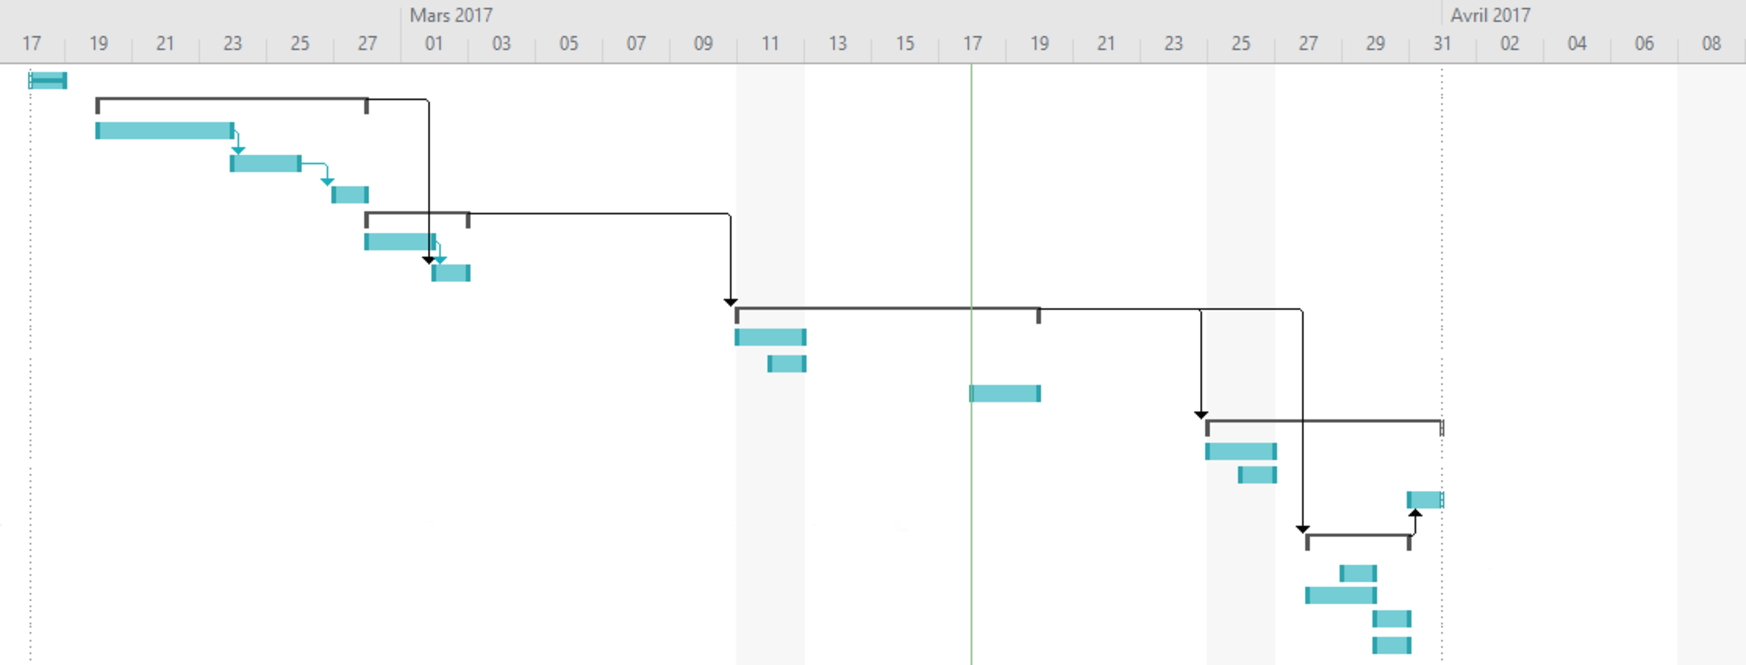
\includegraphics[scale=0.5]{textures/images/diagrammes/DiagrammeDeGantt.pdf}
    \caption{Diagramme de Gantt}
\end{figure}
\begin{figure}[!h]
    \centering
    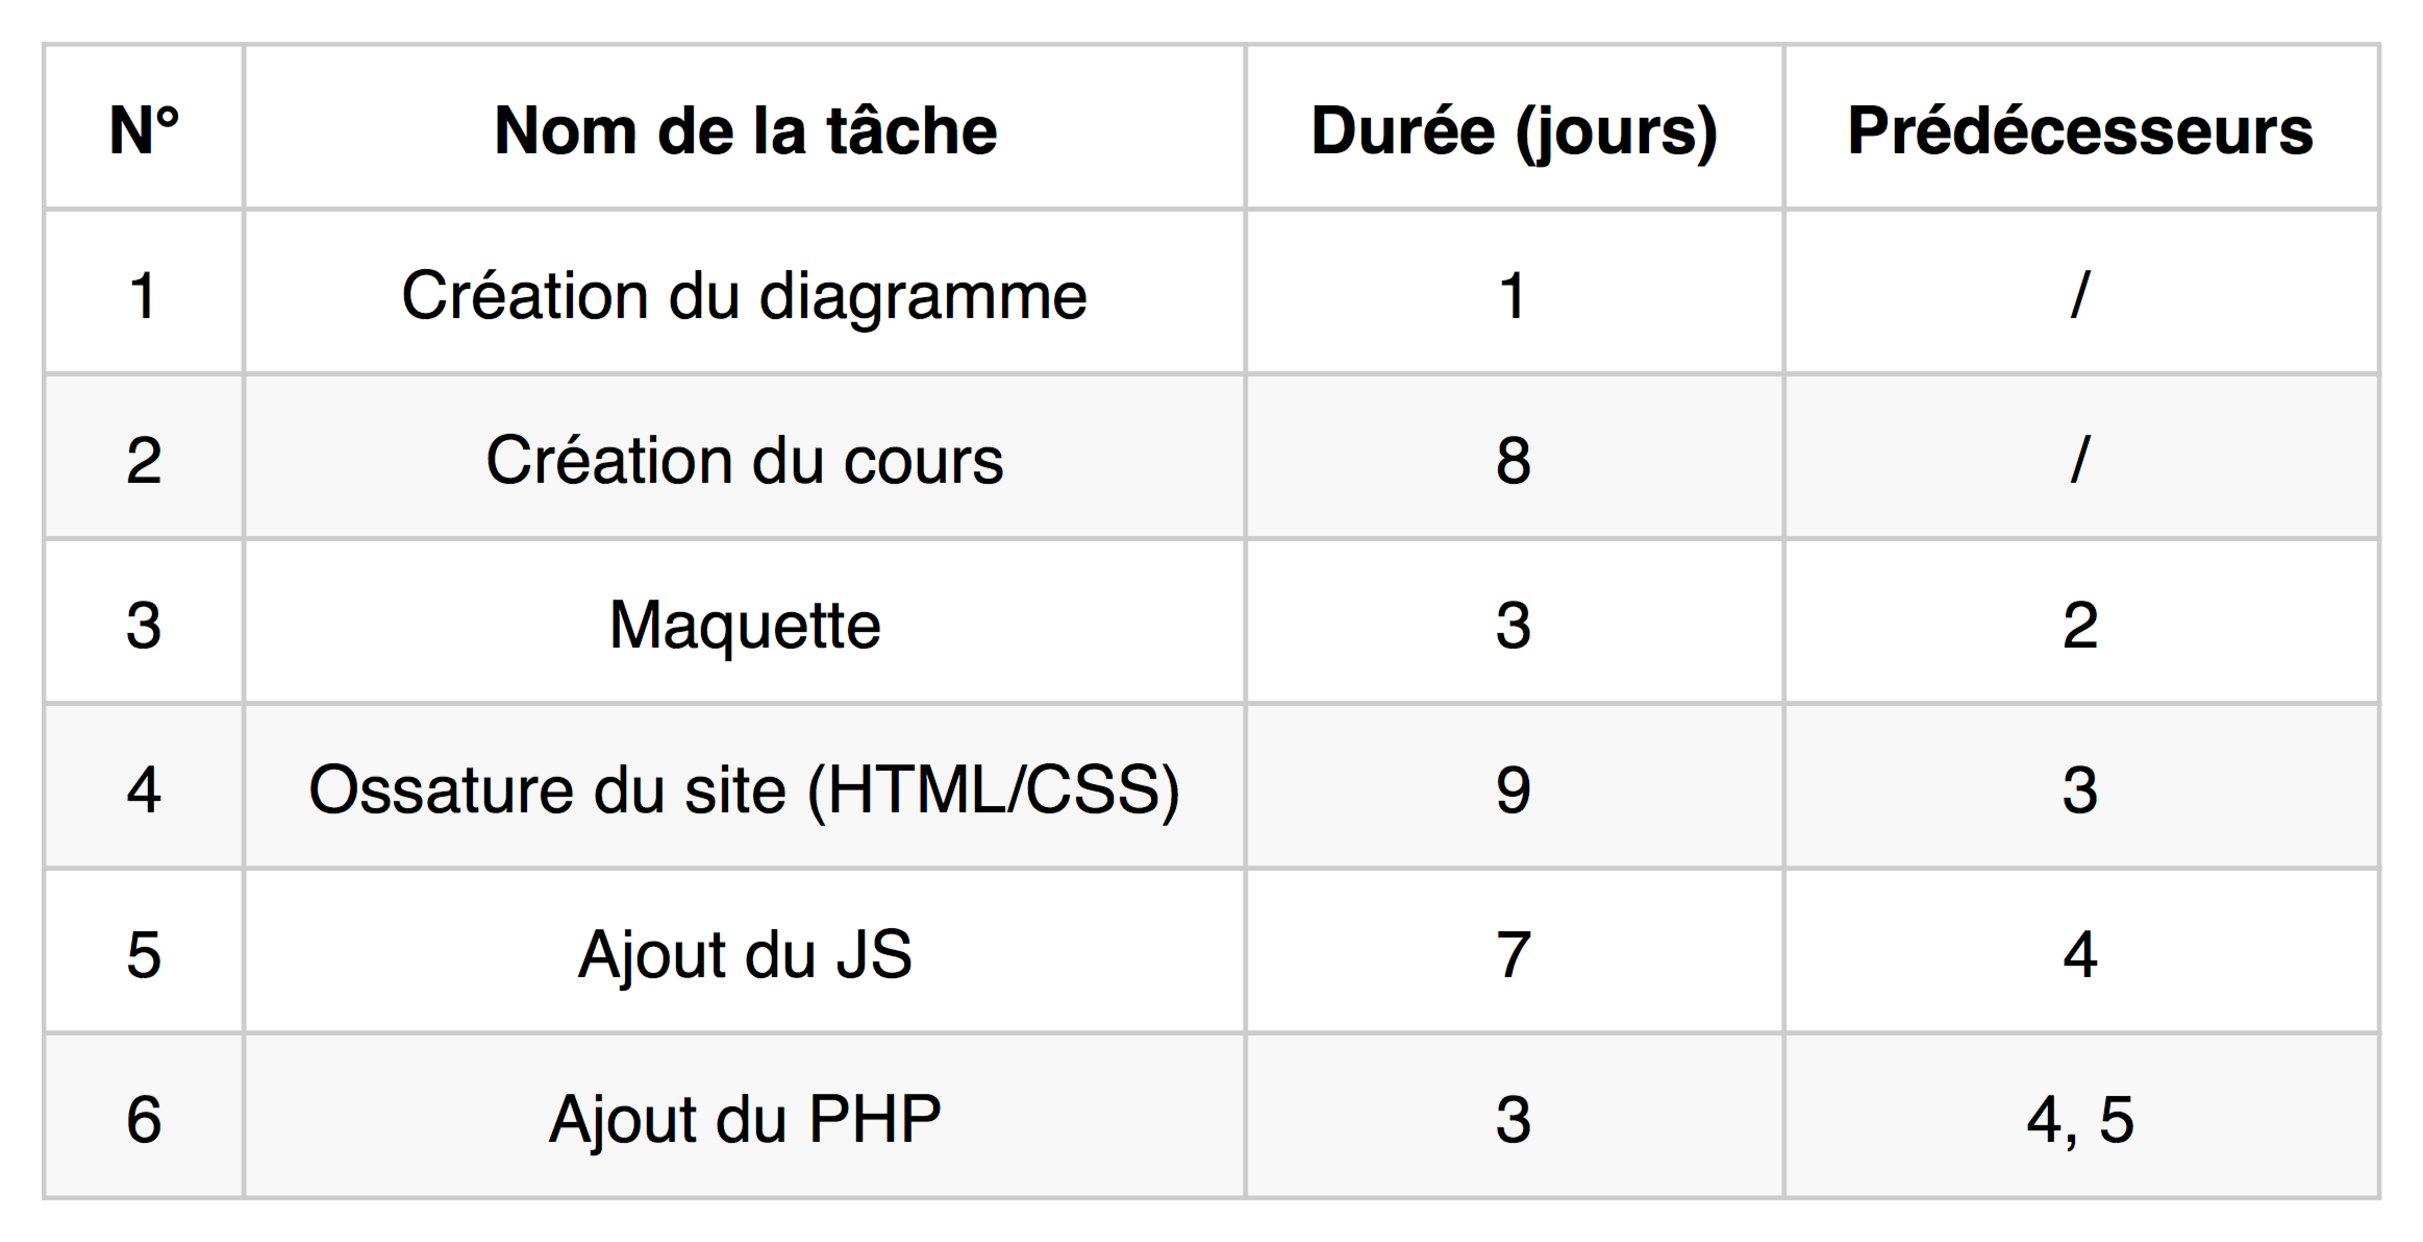
\includegraphics[scale=0.3]{textures/images/diagrammes/TableauDeGantt_brief.pdf}
    \caption{Tableau descriptif}
\end{figure}

Comme on peut le voir, la durée totale prévue du projet est de 31 jours.\\

Le projet est découpé en 6 tâches principales détaillées ci-dessous. \\

La création du diagramme a duré moins d'un jour, mais c'était la durée minimale disponible dans \textit{Microsoft Project}… \\

\newpage

La création du cours comprend l'écriture des différents chapitres et questionnaires. \\
Comme dit précédemment, celle-ci s'est déroulée en deux étapes :
\begin{enumerate}

    \item L'écriture d'un premier jet de trois chapitres : les variables, les booléens et la complexité, et… de quelques exercices.
    \item La réécriture des chapitres sur les variables et les booléens, et l'écriture des autres chapitres \textit{(l'introduction, les conditions et les boucles)}. Chacun accompagné de son questionnaire principal et de ses questionnaires secondaires. \\
    Le questionnaire principal teste, en quatre questions, les connaissances acquises tout au long du chapitre, tandis que les secondaires testent celles de la page précédente en deux questions.\\
    
\end{enumerate}

Cinq maquettes ont été créées :
\begin{enumerate}

    \item La page d'accueil, très \textit{(trop)} simple et sobre;
    \item La page du cours comprenant les liens vers les chapitres;
    \item L'aperçu d'un chapitre. C'est la raison pour laquelle les maquettes dépendent de la tâche précédente;
    \item La page des trophées;
    \item La page du compte de l'utilisateur. \\
    
\end{enumerate}

Dans la version finale, on peut remarquer que le design a évolué. Comme lors d'une démonstration, celui-ci a été jugé \og \textit{trop simple} \fg j'en ai profité pour ajouter des \textbf{animations} sur la page d’accueil, sur les chapitres ainsi que sur les trophées, et de la \textbf{coloration syntaxique} du code. \\

La création de l'ossature du site fut la partie la plus longue parce que la majorité du code du site a été écrite à ce moment. \\
Ainsi, toutes les pages \textit{(accueil, cours, chapitres, trophées, etc.)}, styles et effets CSS ont été créés et n'ont plus été changés depuis. \\

L'ajout du JavaScript est autant lié au code HTML qu'à celui en PHP : il est utilisé dans tout ce qui est animations et boutons. \\
Par exemple, les boutons utilisés pour modifier les données de l'utilisateur ou pour supprimer le compte sont écrits en HTML et CSS. L'action est exécutée en JavaScript et passe par le PHP pour se connecter à la base de données. \\

Pour terminer, l'ajout du PHP a été un gros morceau : le fait de mixer les codes HTML, PHP et MySQL n'a pas été simple. \\
En effet, comme c'est mon premier projet, \textit{en parallèle avec celui du cours de PHP}, à mettre en œuvre un site connecté à une base de données, cela m'a demandé pas mal de travail pour arriver au bon résultat. \\
De plus, sans le PHP, il n'y aurait pas de connexion, d'inscription ou de déblocage des chapitres. Tout cela est directement lié à la base de données, elle-même liée au site par le PHP.

\newpage


\subsection{PERT}
\label{subsec:pert}

Après avoir travaillé le diagramme de Gantt, j'ai réalisé le diagramme de PERT.
Ci-dessous, vous pouvez le voir dans sa forme initiale :

\begin{figure}[h]
  \centering
  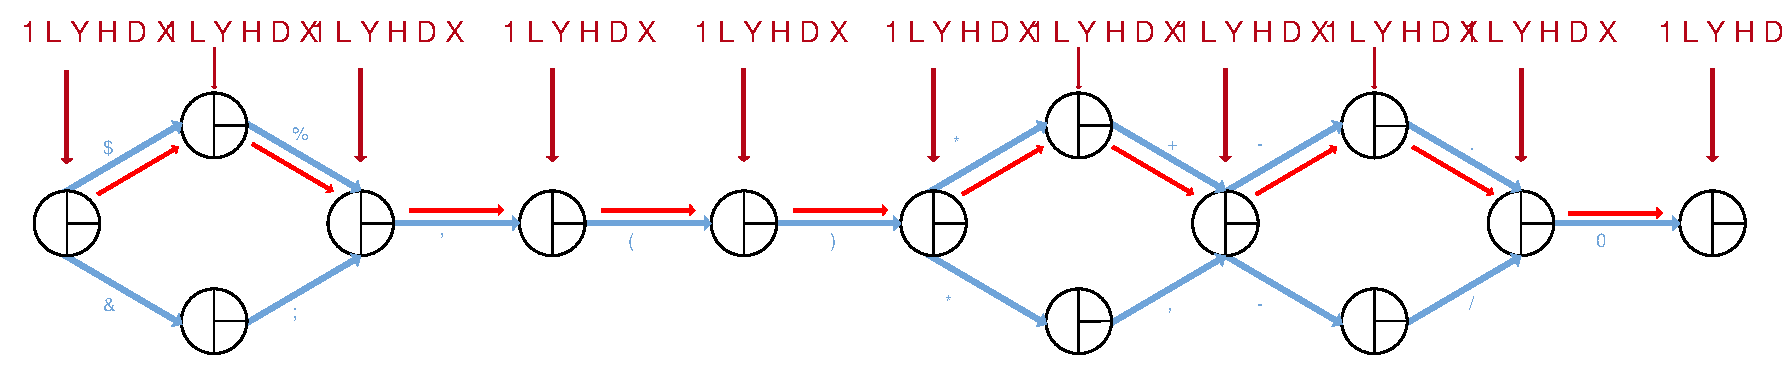
\includegraphics[scale=0.49]
  {textures/images/diagrammes/DiagrammeDePert1.pdf}
  \caption{Diagramme de PERT initial}
  \label{fig:pert-initial}
\end{figure}

Après que le projet soit terminé, j'ai refait le diagramme de PERT afin de coller au plus près au temps passé sur les différentes tâches :

\begin{figure}[h]
  \centering
  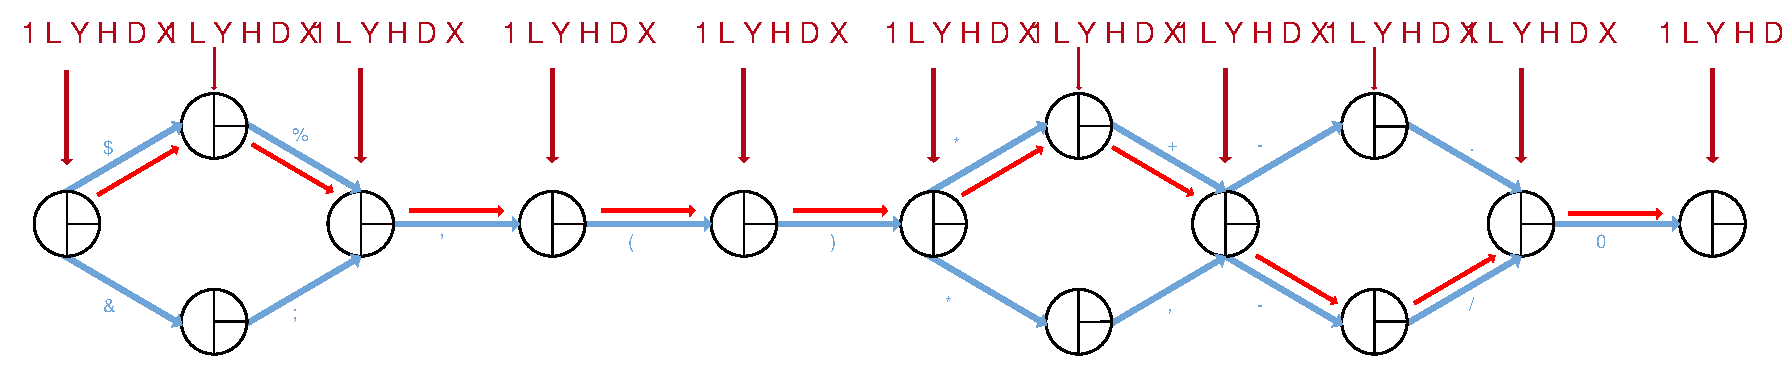
\includegraphics[scale=0.49]
  {textures/images/diagrammes/DiagrammeDePert2.pdf}
  \caption{Diagramme de PERT final}
  \label{fig:pert-final}
\end{figure}

La première chose que l'on peut remarquer, c'est qu'il a fallu moins de temps que prévu pour terminer le projet \textit{(on passe de \textbf{29h15} à \textbf{27h})}. \\

Dans ce diagramme, les tâches sont plus nombreuses pour plus de précision, et leur durée est plus juste. On parle désormais en heures et plus en jours. \\
Par exemple, on peut voir que l'écriture des chapitres dure 8 heures et que celle des exercices en dépend. \\
De même pour la création de la maquette qui ne dépend plus entièrement des tâches ci-dessus. C'est la tâche \textbf{D}, le test de la maquette avec le texte, qui dépend de l'existence du cours, et elle ne dure qu'un quart d'heure.

\newpage

Voici le tableau des antériorités lié au diagramme final :

\begin{figure}[h]
  \centering
  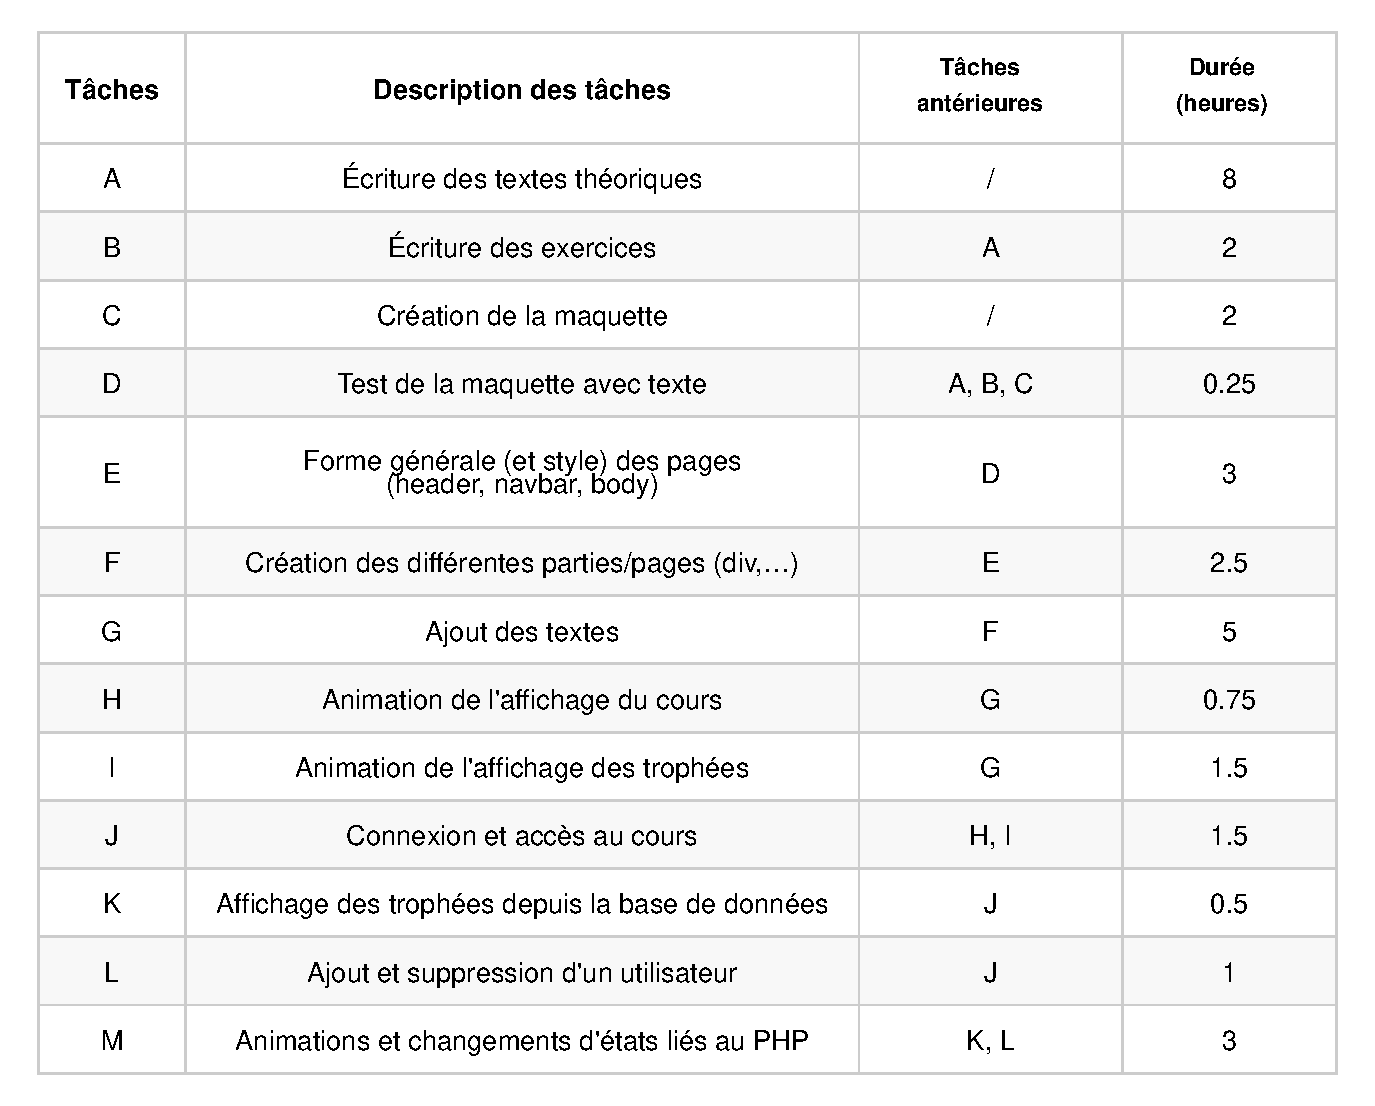
\includegraphics[scale=0.6]
  {textures/images/diagrammes/TableauDesAnteriorites.pdf}
  \caption{Tableau des antériorités}
  \label{fig:tableau-anteriorites}
\end{figure}


{\Large \textbf{Différences entre l'initial et le final}}

Jusqu'à la tâche \textbf{F}, \textit{niveau 7}, il n'y a pas de différences. \\
Après celle-ci, quatre des sept tâches ont eu des durées différentes de ce que j'avais escompté :

\begin{enumerate}

    \item la tâche \textbf{G} est passée de \textbf{1h30} à \textbf{5h}. La cause est simple, la mise en page des chapitres a été plus complexe que prévu.
    En cause, l'ajout de coloration syntaxique, l'ajout de styles pour les types \textit{(gras, italique, etc.)}, ainsi que l'ajout d'un slider \footnote{\url{http://callmenick.com/post/responsive-content-slider}} divisant les chapitres en différentes parties, etc.
    
    \item la connexion à la base de données, tâche \textbf{J}, a pris moins de temps que prévu. \\
    \textbf{Remarquons}, tout de même, que de nombreux changements à ce niveau ont été effectués à la tâche \textbf{M}, dont la raison d'être était de résoudre les problèmes potentiels.
    
    \item l'affichage du résultat dans les trophées \textit{depuis la base de données}, \textit{la tâche \textbf{K}}, a été beaucoup moins difficile qu'imaginé grâce à l'avancée du projet du cours de \textit{Programmation web}.
    
    \item il en est de même pour la tâche \textbf{L}, \textit{l'ajout et la suppression d'utilisateurs}, a donc pris moins de temps.

\end{enumerate}

%%% Local Variables:
%%% mode: latex
%%% TeX-master: t
%%% End:

    \newpage
    \section{Base de données}
\label{sec:BD}


\subsection{Création de la base de données}
\label{subsec:creation-db}

La base de données est composée de trois tables contenant toutes les données utiles au bon fonctionnement du site.\\
Il y a la table \textbf{Users} \textit{pour tout ce qui concerne les utilisateurs}, la table \textbf{Results}, \textit{qui concerne les résultats de chaque chapitre} et la table \textbf{Tests} \textit{qui contient la liste des résultats}.

\begin{figure}[h]
  \centering
  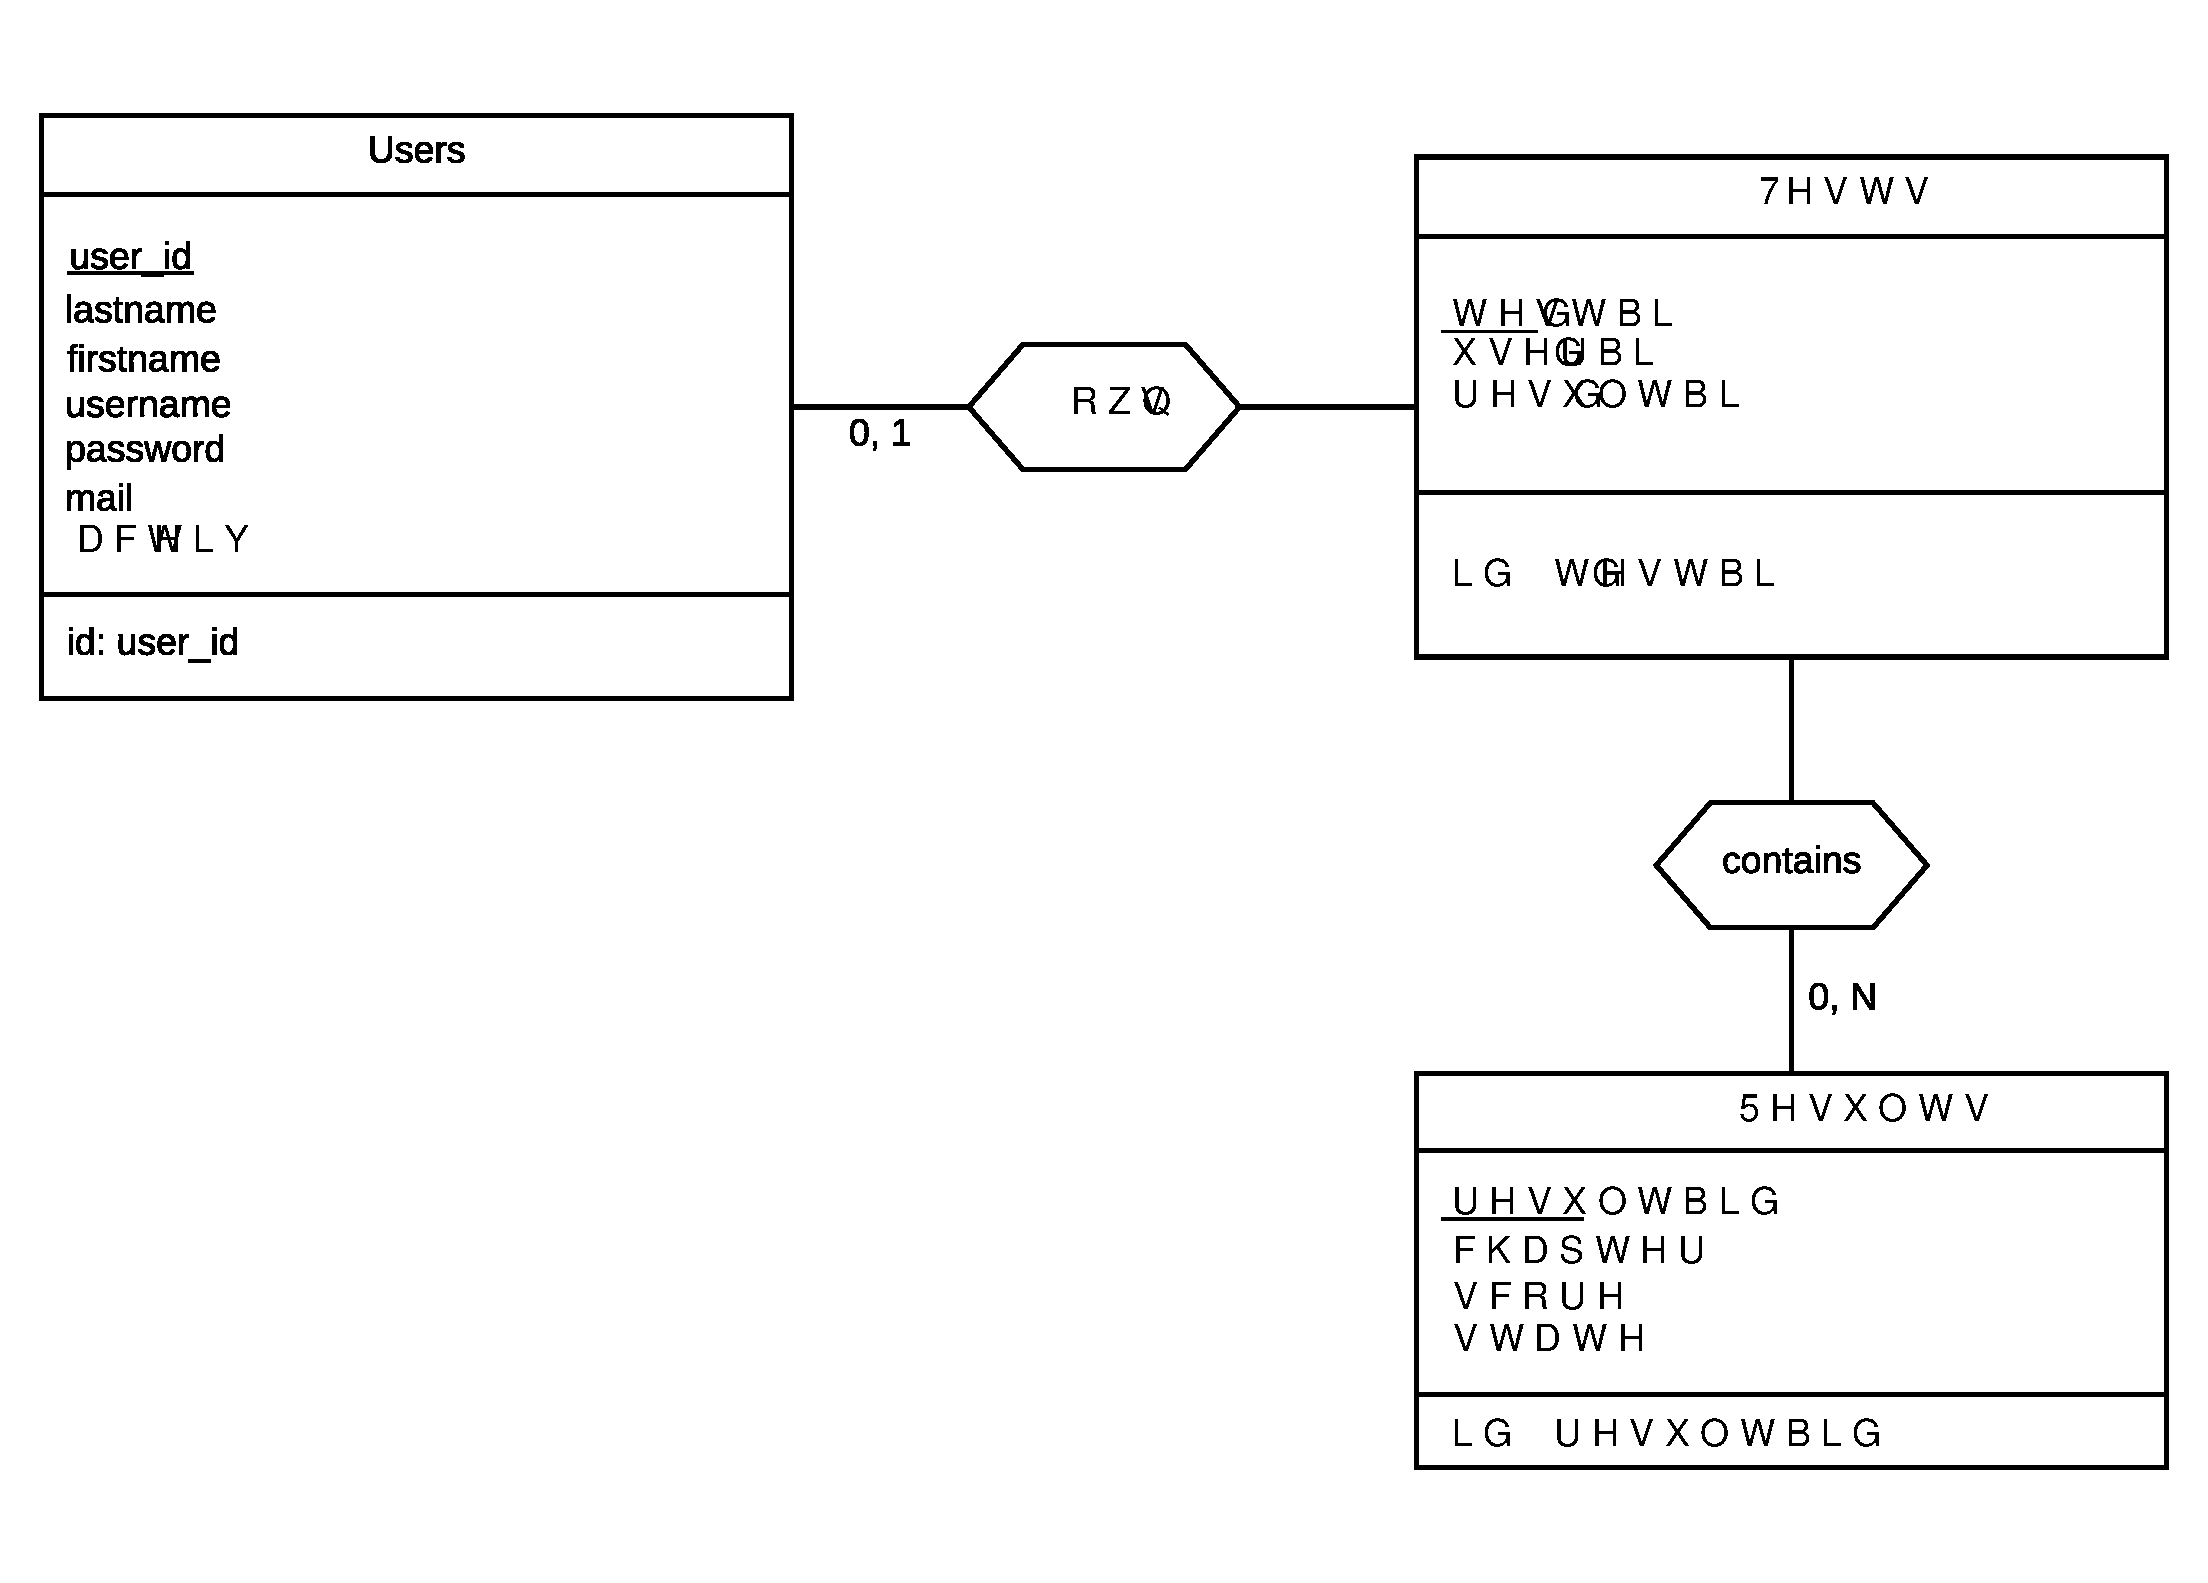
\includegraphics[scale=0.4]
  {textures/images/DB/DB.pdf}
  \caption{Schéma conceptuel de la base de données}
  \label{fig:db}
\end{figure}

\newpage


\subsection{Connexion à la base de données}
\label{subsec:conn-bd}

Le type de requêtes utilisé pour l'accès à la base de données est le type PDO.\\
De manière plus précise, ce sont des requêtes préparées qui ont été utilisées pour plus de sécurité \textit{(voir la section~\ref{subsec:securite}\textbf{~\nameref{subsec:securite}})}.\\
De plus, PDO permet plus de flexibilité. Elle est recommandée, très utilisée \textit{(et possède donc une importante communauté)} et est enseignée à l'école.\\

On pourrait alors ajouter, dans les évolutions possibles, le passage à la \textit{programmation orientée objet}, couplée à l’utilisation du \textit{singleton} et, comme structure de site, l’utilisation du \textit{design pattern \textbf{MVC}}.


\subsection{Sécurité}
\label{subsec:securite}

Pour la sécurité du site, tout accès à la base de données passe par des requêtes préparées \textit{(PDO)}, car celles-ci le protègent de toute injection SQL.\\

La connexion au site est surveillée grâce à la mise en place d’une session. Dès qu’un accès à une page se fait, la connexion est vérifiée. Si l’utilisateur n’est pas identifié, il est redirigé vers la page d’accueil.\\

En plus de cela, chaque champ de formulaire est protégé par des \textit{regex}\footnote{\href{https://fr.wikipedia.org/wiki/Expression\_rationnelle}{Expression régulière (en anglais: \textbf{Reg}ular \textbf{ex}pression)}}.\\
Celles-ci vérifient que les données entrées sont de la forme voulue: un nom ne doit contenir que des lettres et, selon une certaine forme, peut être divisé à l’aide d’un trait d’union; une adresse mail ne contient que des lettres minuscules non-accentuées, des points et un seul arobase; etc.\\

De plus, les mots de passe ont une longueur minimale de quatre caractères et doivent contenir, au moins, une majuscule, une minuscule et un chiffre.\\
Ils sont aussi \textit{hachés}\footnote{\url{https://fr.wikipedia.org/wiki/Fonction\_de\_hachage\_cryptographique}} à l’aide de \textit{SHA512} et d’un \textit{salage dynamique} pour plus de sécurité.\\
En effet, le mot de passe est de la forme \textbf{+\%\# longueur mot\_de\_passe  ¨*§}.\\ Par exemple, le mot de passe \textbf{Test1} devient \textbf{+\%\#5Test1¨*§} avant d’être haché.\\
Il est ainsi indéchiffrable, mais cela a aussi pour effet de sécuriser la base de données puisque le résultat ne contiendra que des caractères sûrs.



%%% Local Variables:
%%% mode: latex
%%% TeX-master: t
%%% End:
    \newpage
    \section{Conclusion}
\label{sec:conclusion}

Le projet que j'ai choisi est un site qui permet d’apprendre les bases de la programmation en Python. \\

Un utilisateur, identifié par son nom d’utilisateur, peut modifier ses données depuis la page \textit{Compte}. \\
Il peut ajouter son nom de famille, son prénom et son adresse mail, et même modifier son mot de passe. \\
Il a aussi la possibilité de supprimer son compte. \\

Pour l'instant, cinq chapitres sont disponibles : \textit{l'introduction}, \textit{les variables}, \textit{les booléens}, \textit{les conditions} et \textit{les boucles}. \\
Le premier est débloqué d'office et, pour débloquer le suivant, il faut réussir le test de fin de chapitre avec une cote minimale de 7/10. \\
En cas d'échec, il faudra revoir le chapitre et repasser le test. \\
L'utilisateur peut retrouver le résultat de chaque chapitre sur la page des trophées. \\

L'acquisition de trophées donne une meilleure dynamique à l'apprentissage de la programmation et permet d'être certain de la bonne compréhension de chaque chapitre avant de passer au suivant. \\

Il est à remarquer que, d’après les bonnes pratiques des bases de données, il ne faut pas supprimer les données mais les rendre invisibles aux utilisateurs. \\
Cette méthode est utilisée lors de la suppression d’un compte qui n’est pas supprimé, mais simplement désactivé. \\

Le projet a été divisé en différentes tâches grâce à l'utilisation des diagrammes de Gant et de PERT. Ce qui offre plus de clarté sur le développement du projet. \\

Lorsque tous les trophées ont été obtenus, l'utilisateur a appris la programmation en Python. L'objectif de ce projet est donc atteint.\\
Mon projet n'est pas que théorique. En effet, il a aussi un but pédagogique. \\
Il m'a permis d'apprendre et d'appliquer les cours reçus, et donc à en voir l'utilité.

%%% Local Variables:
%%% mode: latex
%%% TeX-master: t
%%% End:
    \newpage
    \phantomsection
    \nocite{*}
\addcontentsline{toc}{section}{Références}

\begin{category}{Livres}
    \SBentries{algo}
    \SBentries{cHeH}
    \SBentries{csHeH}
    \SBentries{cZero}
    \SBentries{javaZero}
    \SBentries{latex}
    \SBentries{mor}
\end{category}

\begin{category}{Internet}
    \SBentries{website:bootstrap}
    \SBentries{website:laravel}
    \SBentries{website:pythonWiki}
    \SBentries{website:pythonZero}
    \SBentries{website:slider}
    \SBentries{website:xDupre}
\end{category}

\bibliographystyle{acm} 
\bibliography{bibli}


    \newpage
    \startcontents
\chapter*{Table des annexes}
\addstarredchapter{Annexes}
\label{ch:annexes}
\minitoc
\printcontents{}{1}{}
\setcounter{section}{0}

\newpage
\section*{Les maquettes}
\addcontentsline{ptc}{section}{Les maquettes}
\label{sec:maquettes}

Voici les différentes maquettes du site :

\begin{figure}[!h]
    \centering
    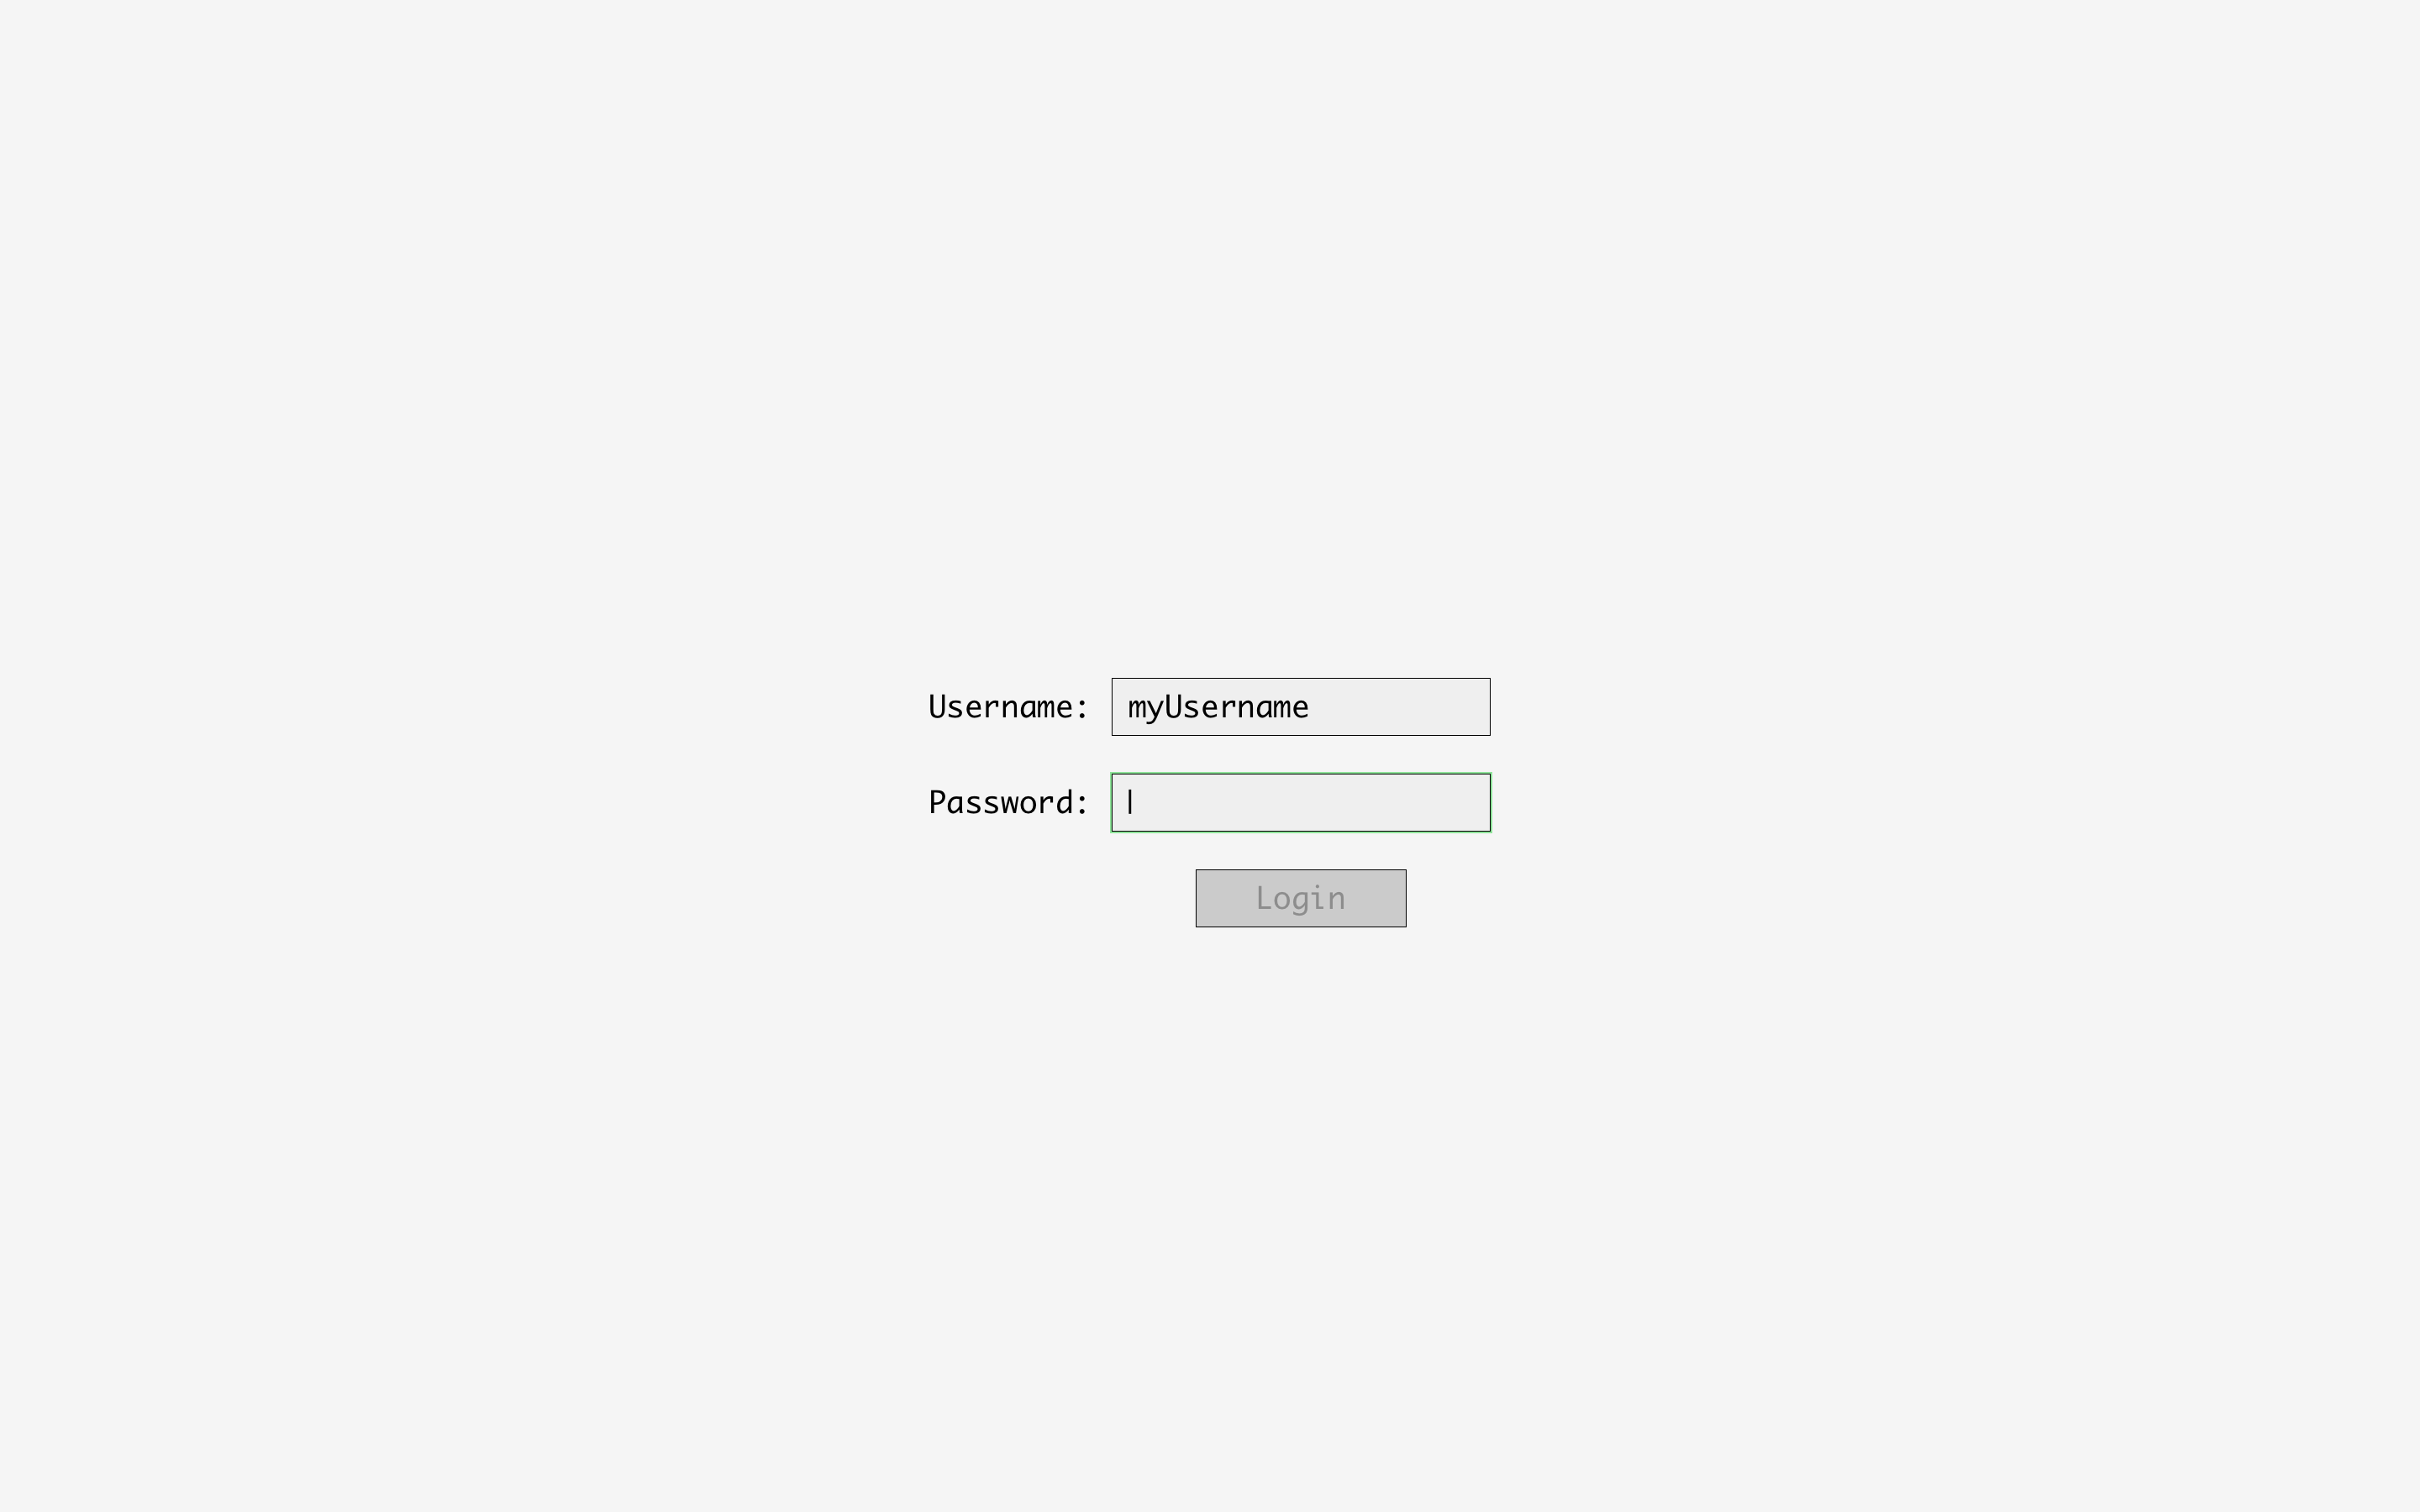
\includegraphics[scale=0.14]{textures/images/annexes/maquettes/1-Login.png}
    \caption{La page d'accueil}
\end{figure}
\begin{figure}[!h]
    \centering
    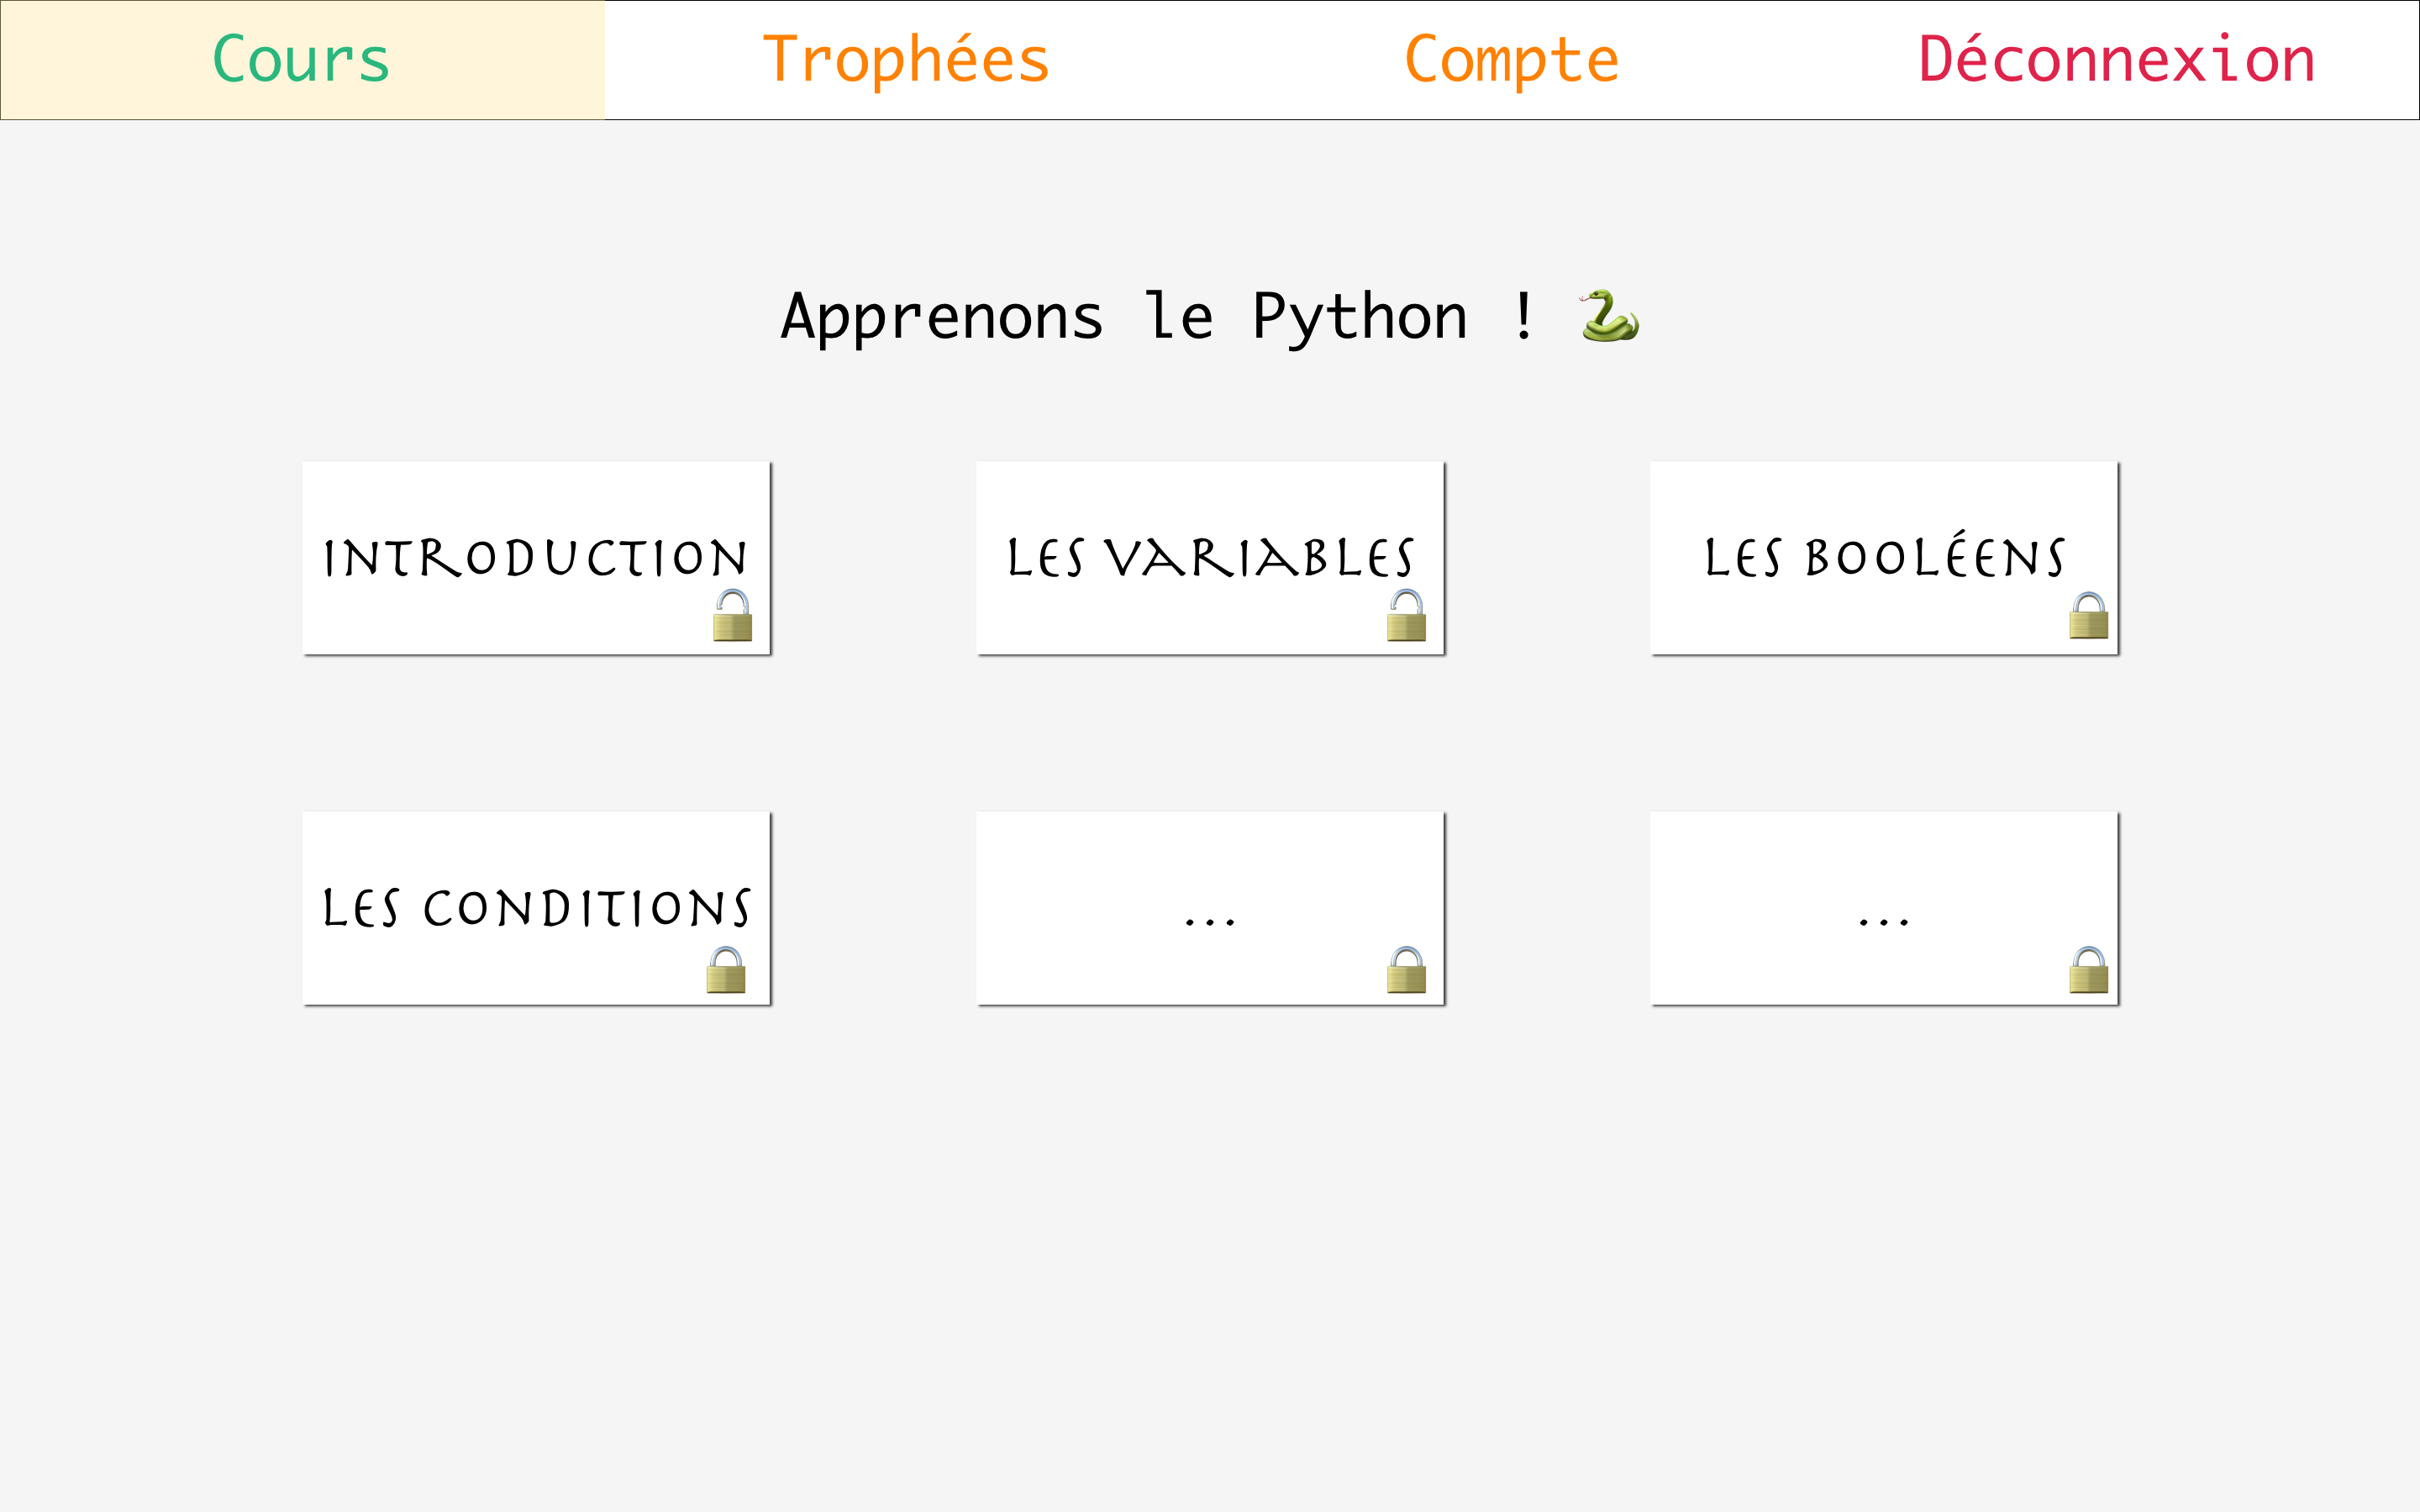
\includegraphics[scale=0.14]{textures/images/annexes/maquettes/21-Sommaire.png}
    \caption{La page de cours}
\end{figure}

\newpage

\begin{figure}[!h]
    \centering
    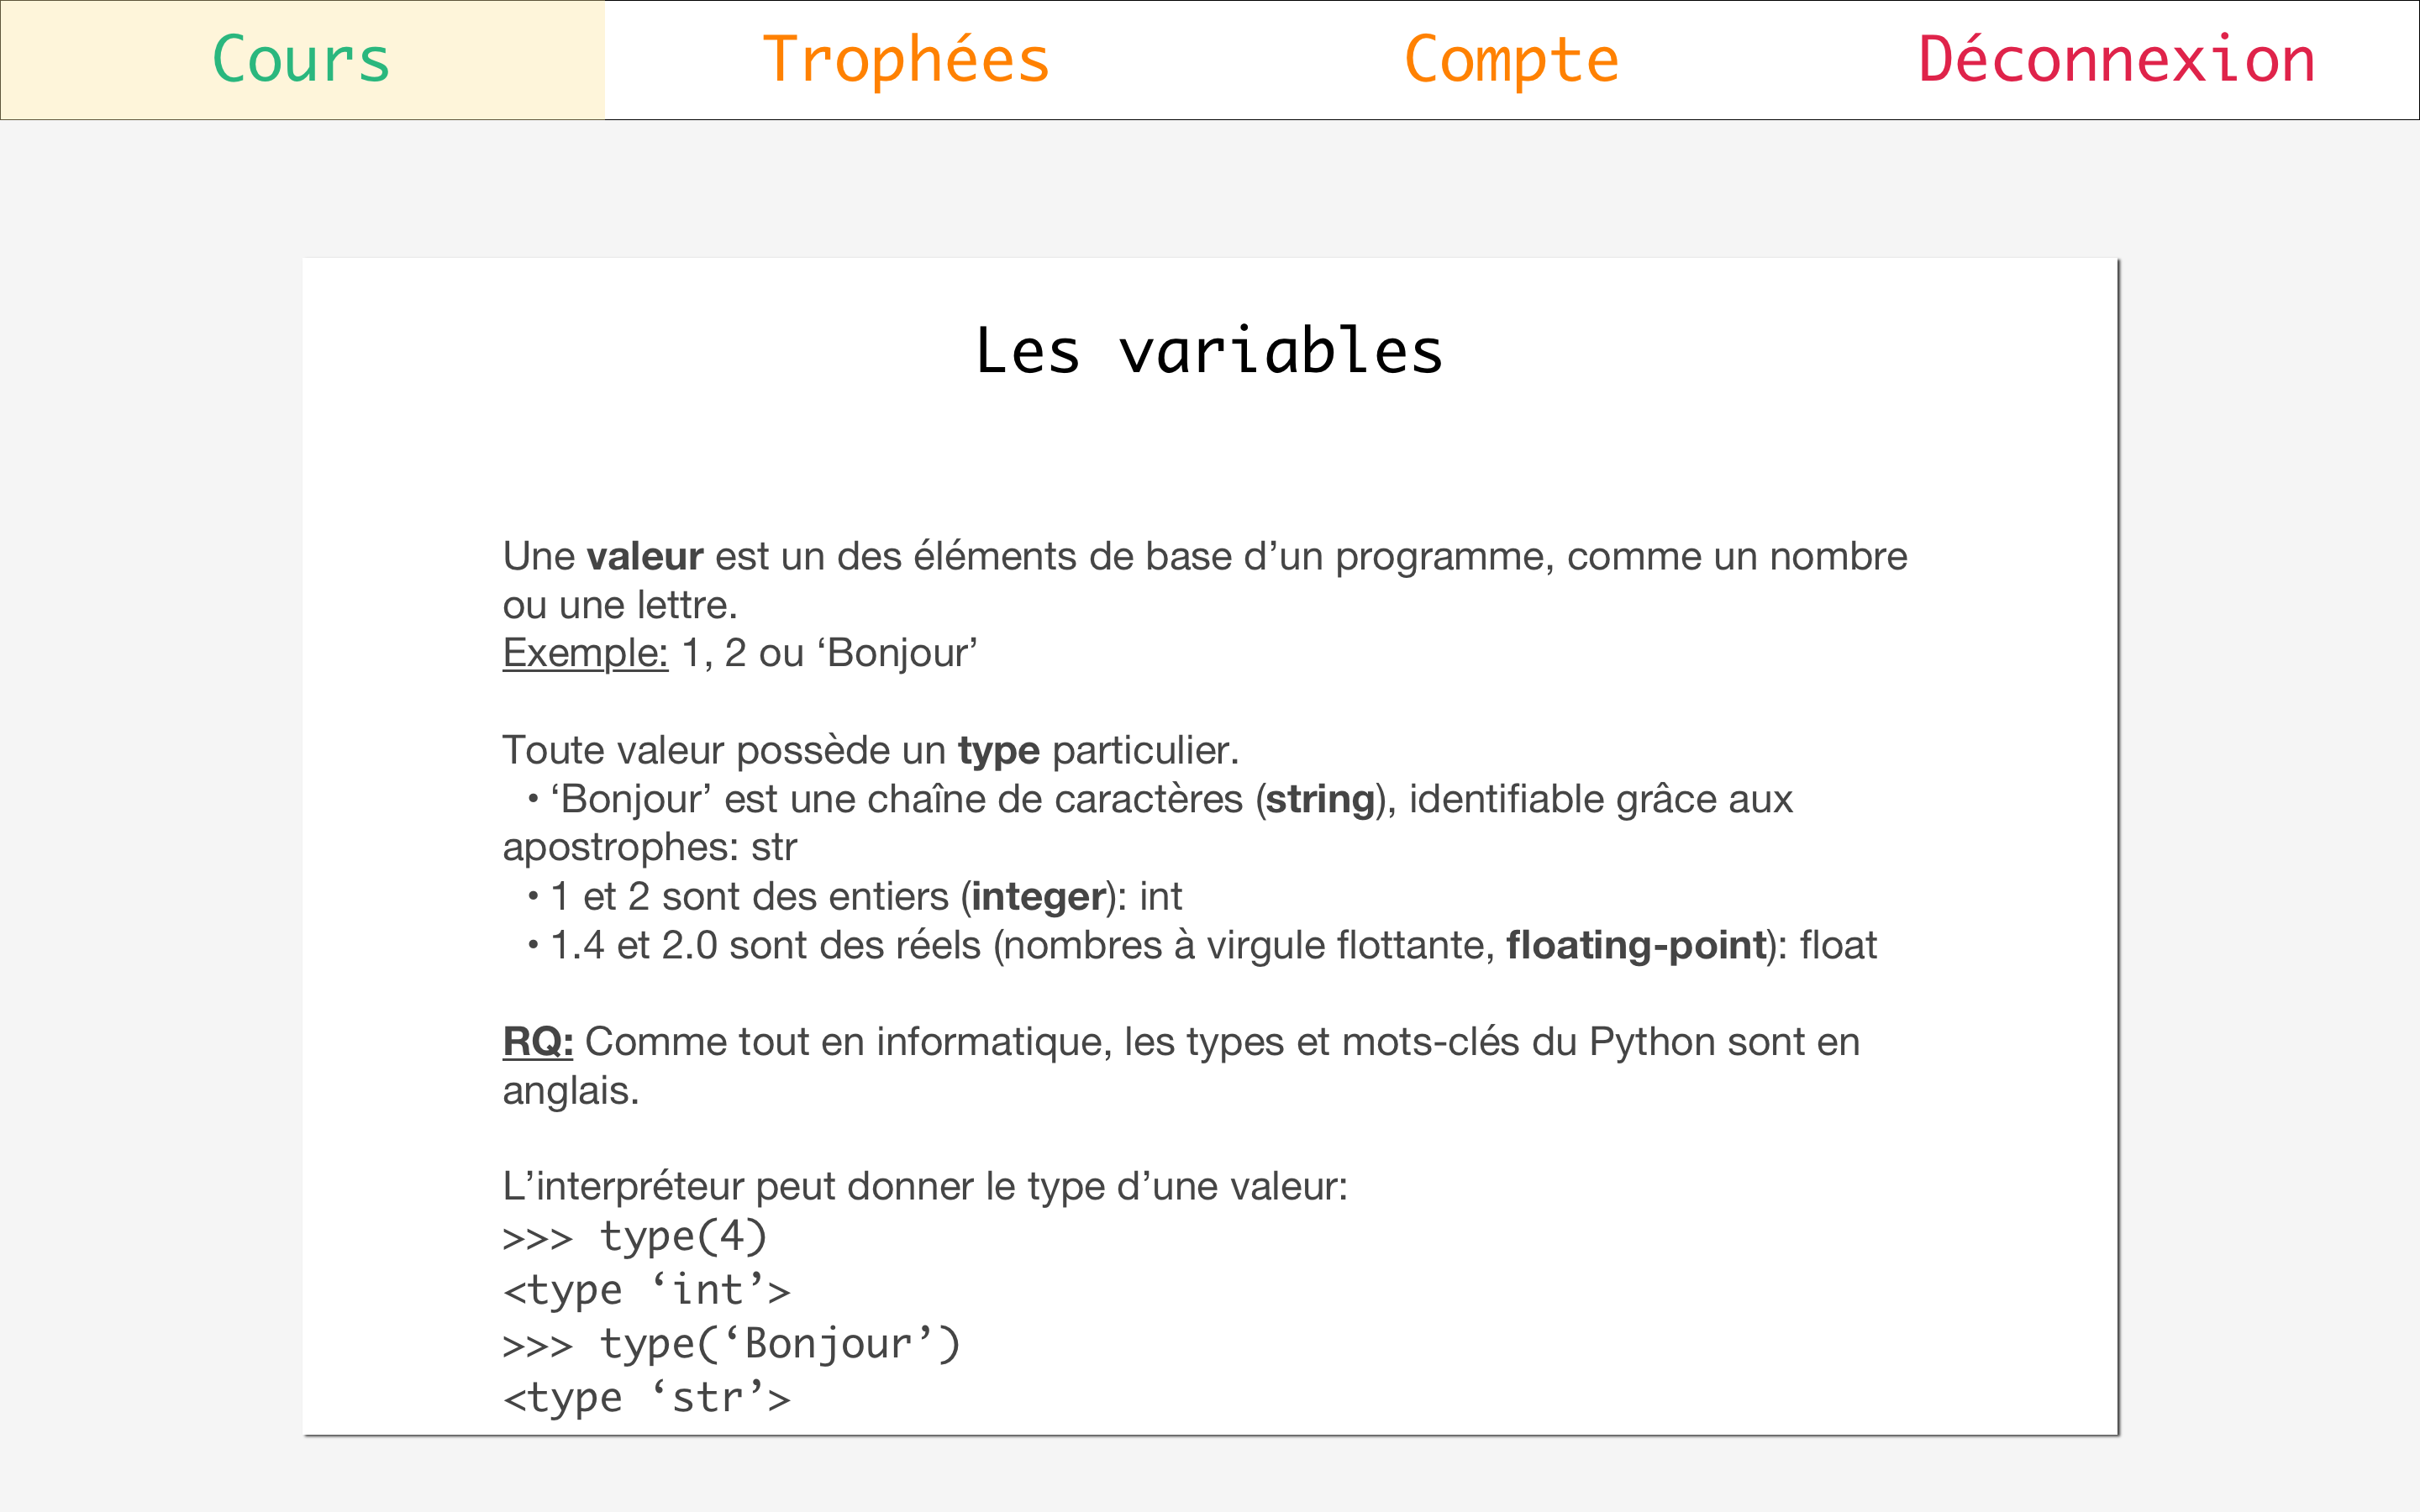
\includegraphics[scale=0.14]{textures/images/annexes/maquettes/22-Cours.png}
    \caption{L'aperçu d'un chapitre}
\end{figure}
\begin{figure}[!h]
    \centering
    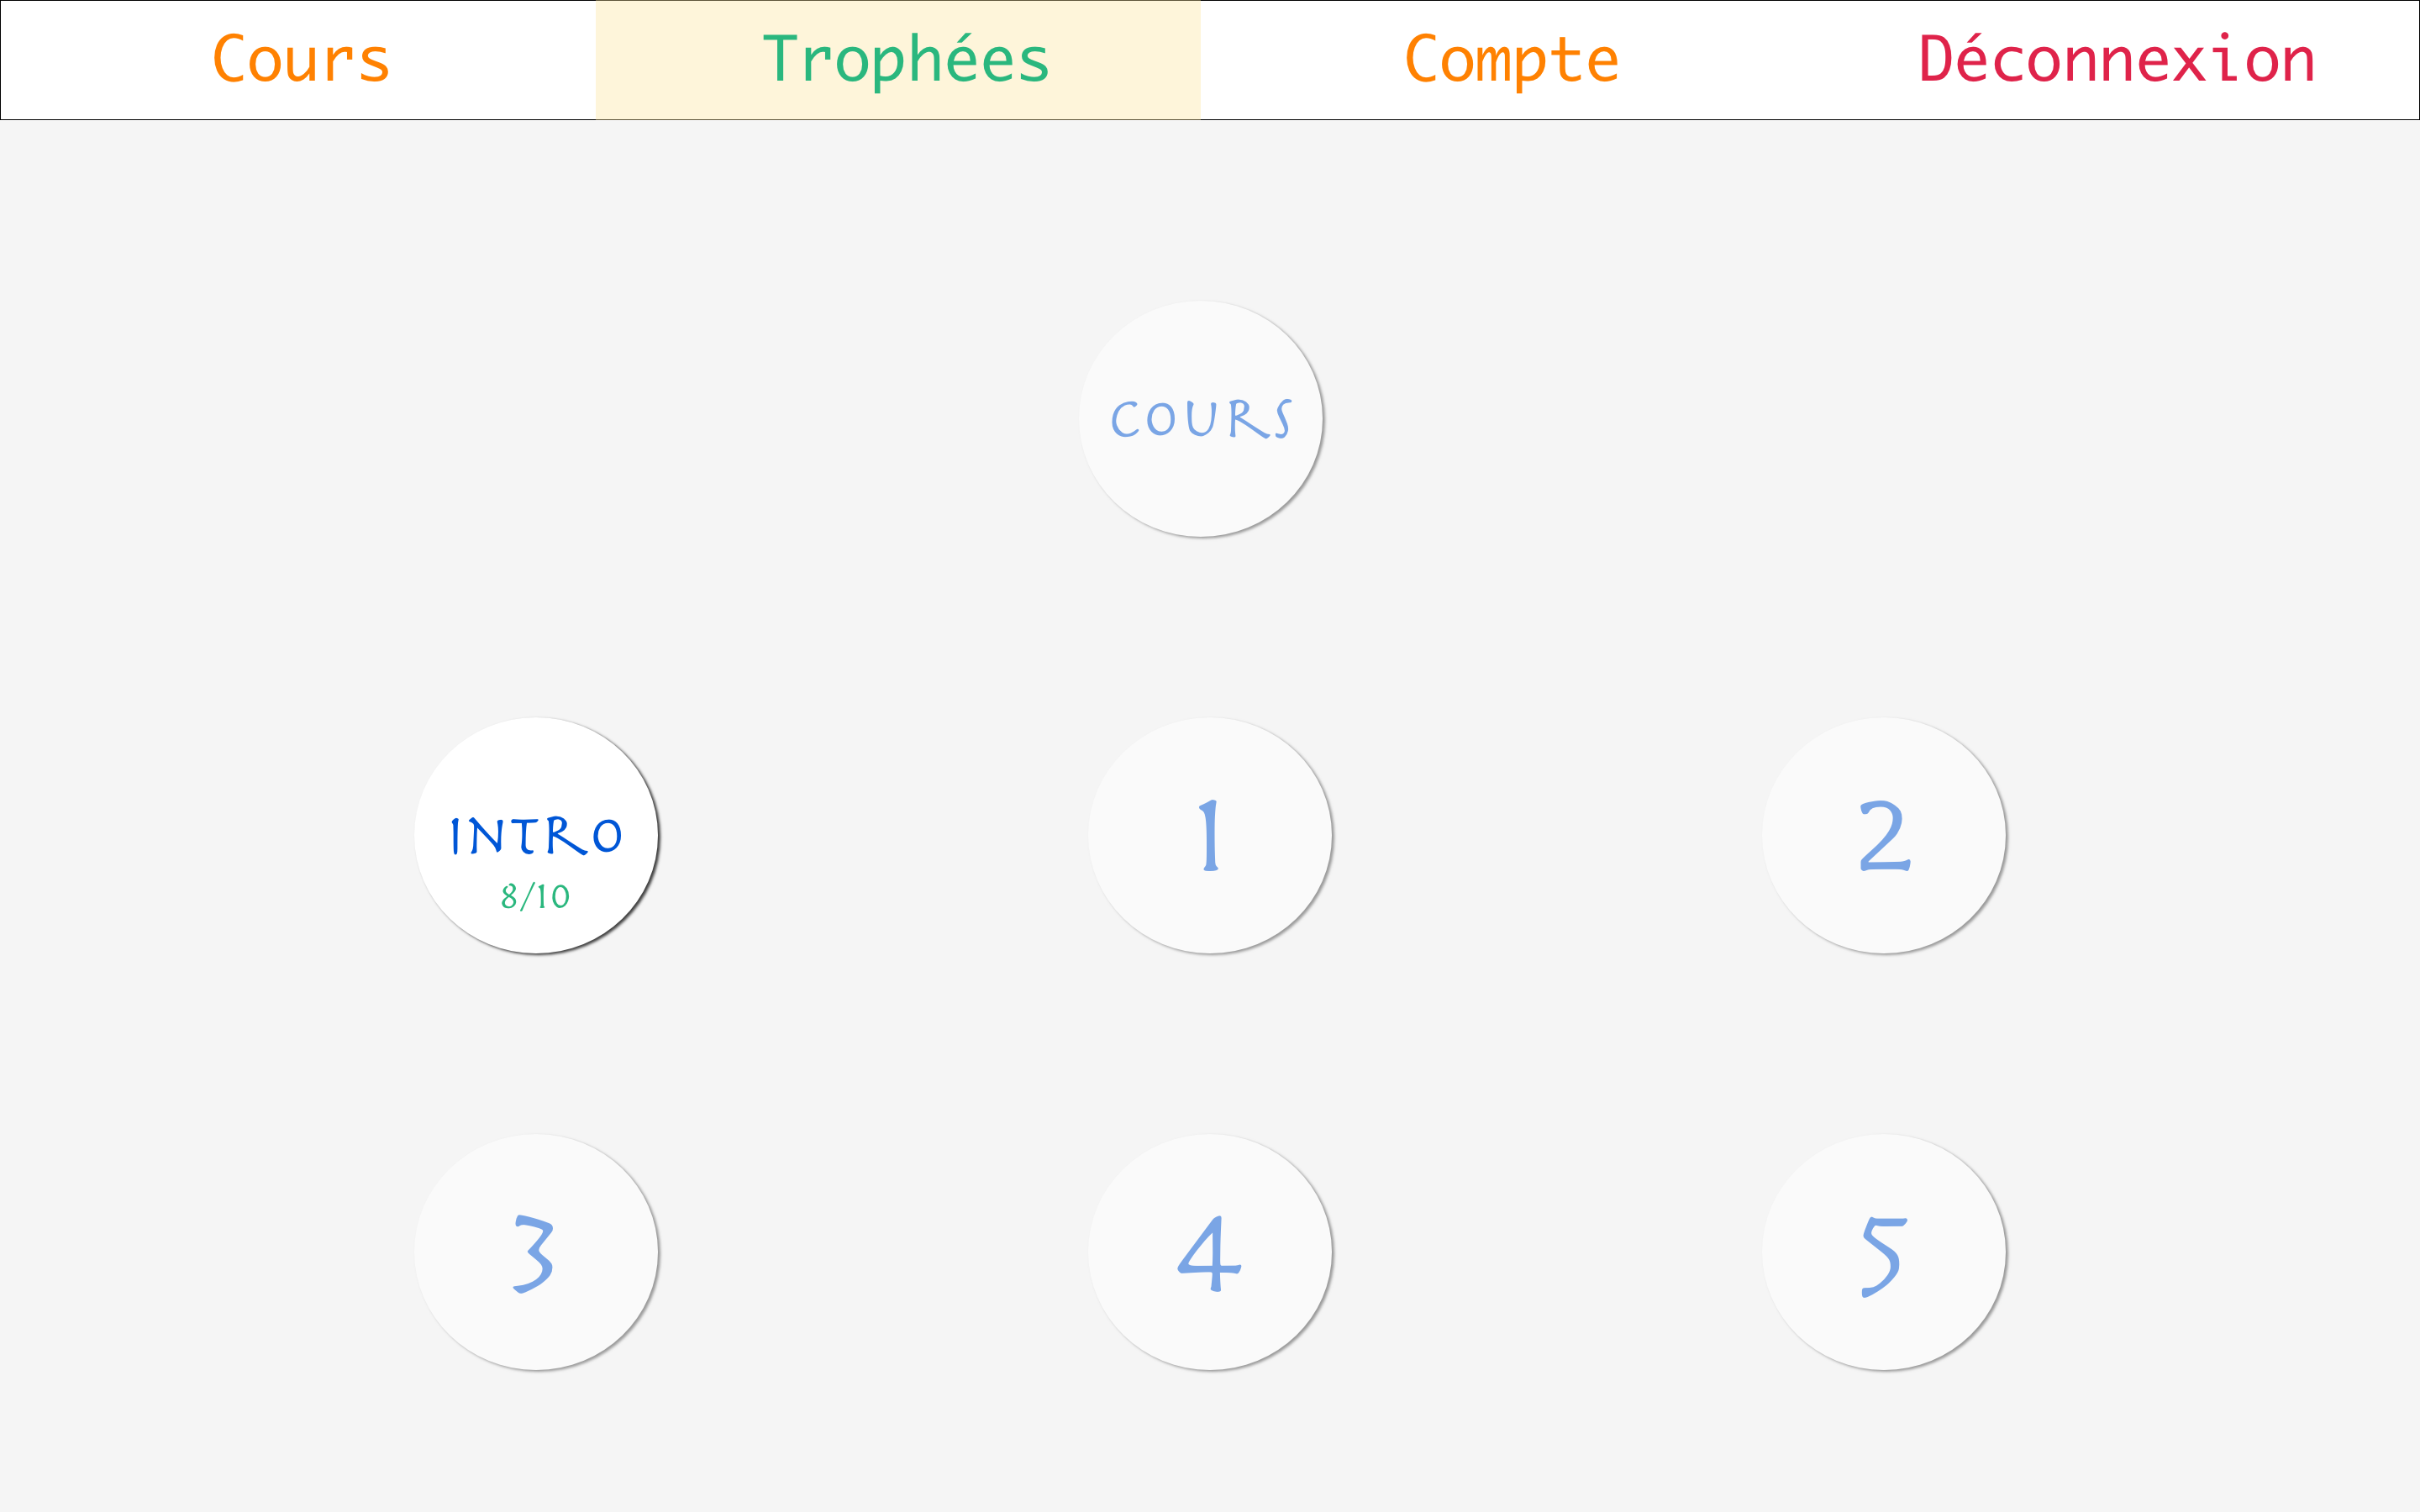
\includegraphics[scale=0.14]{textures/images/annexes/maquettes/3-Trophees.png}
    \caption{La page des trophées}
\end{figure}

\newpage

\begin{figure}[!h]
    \centering
    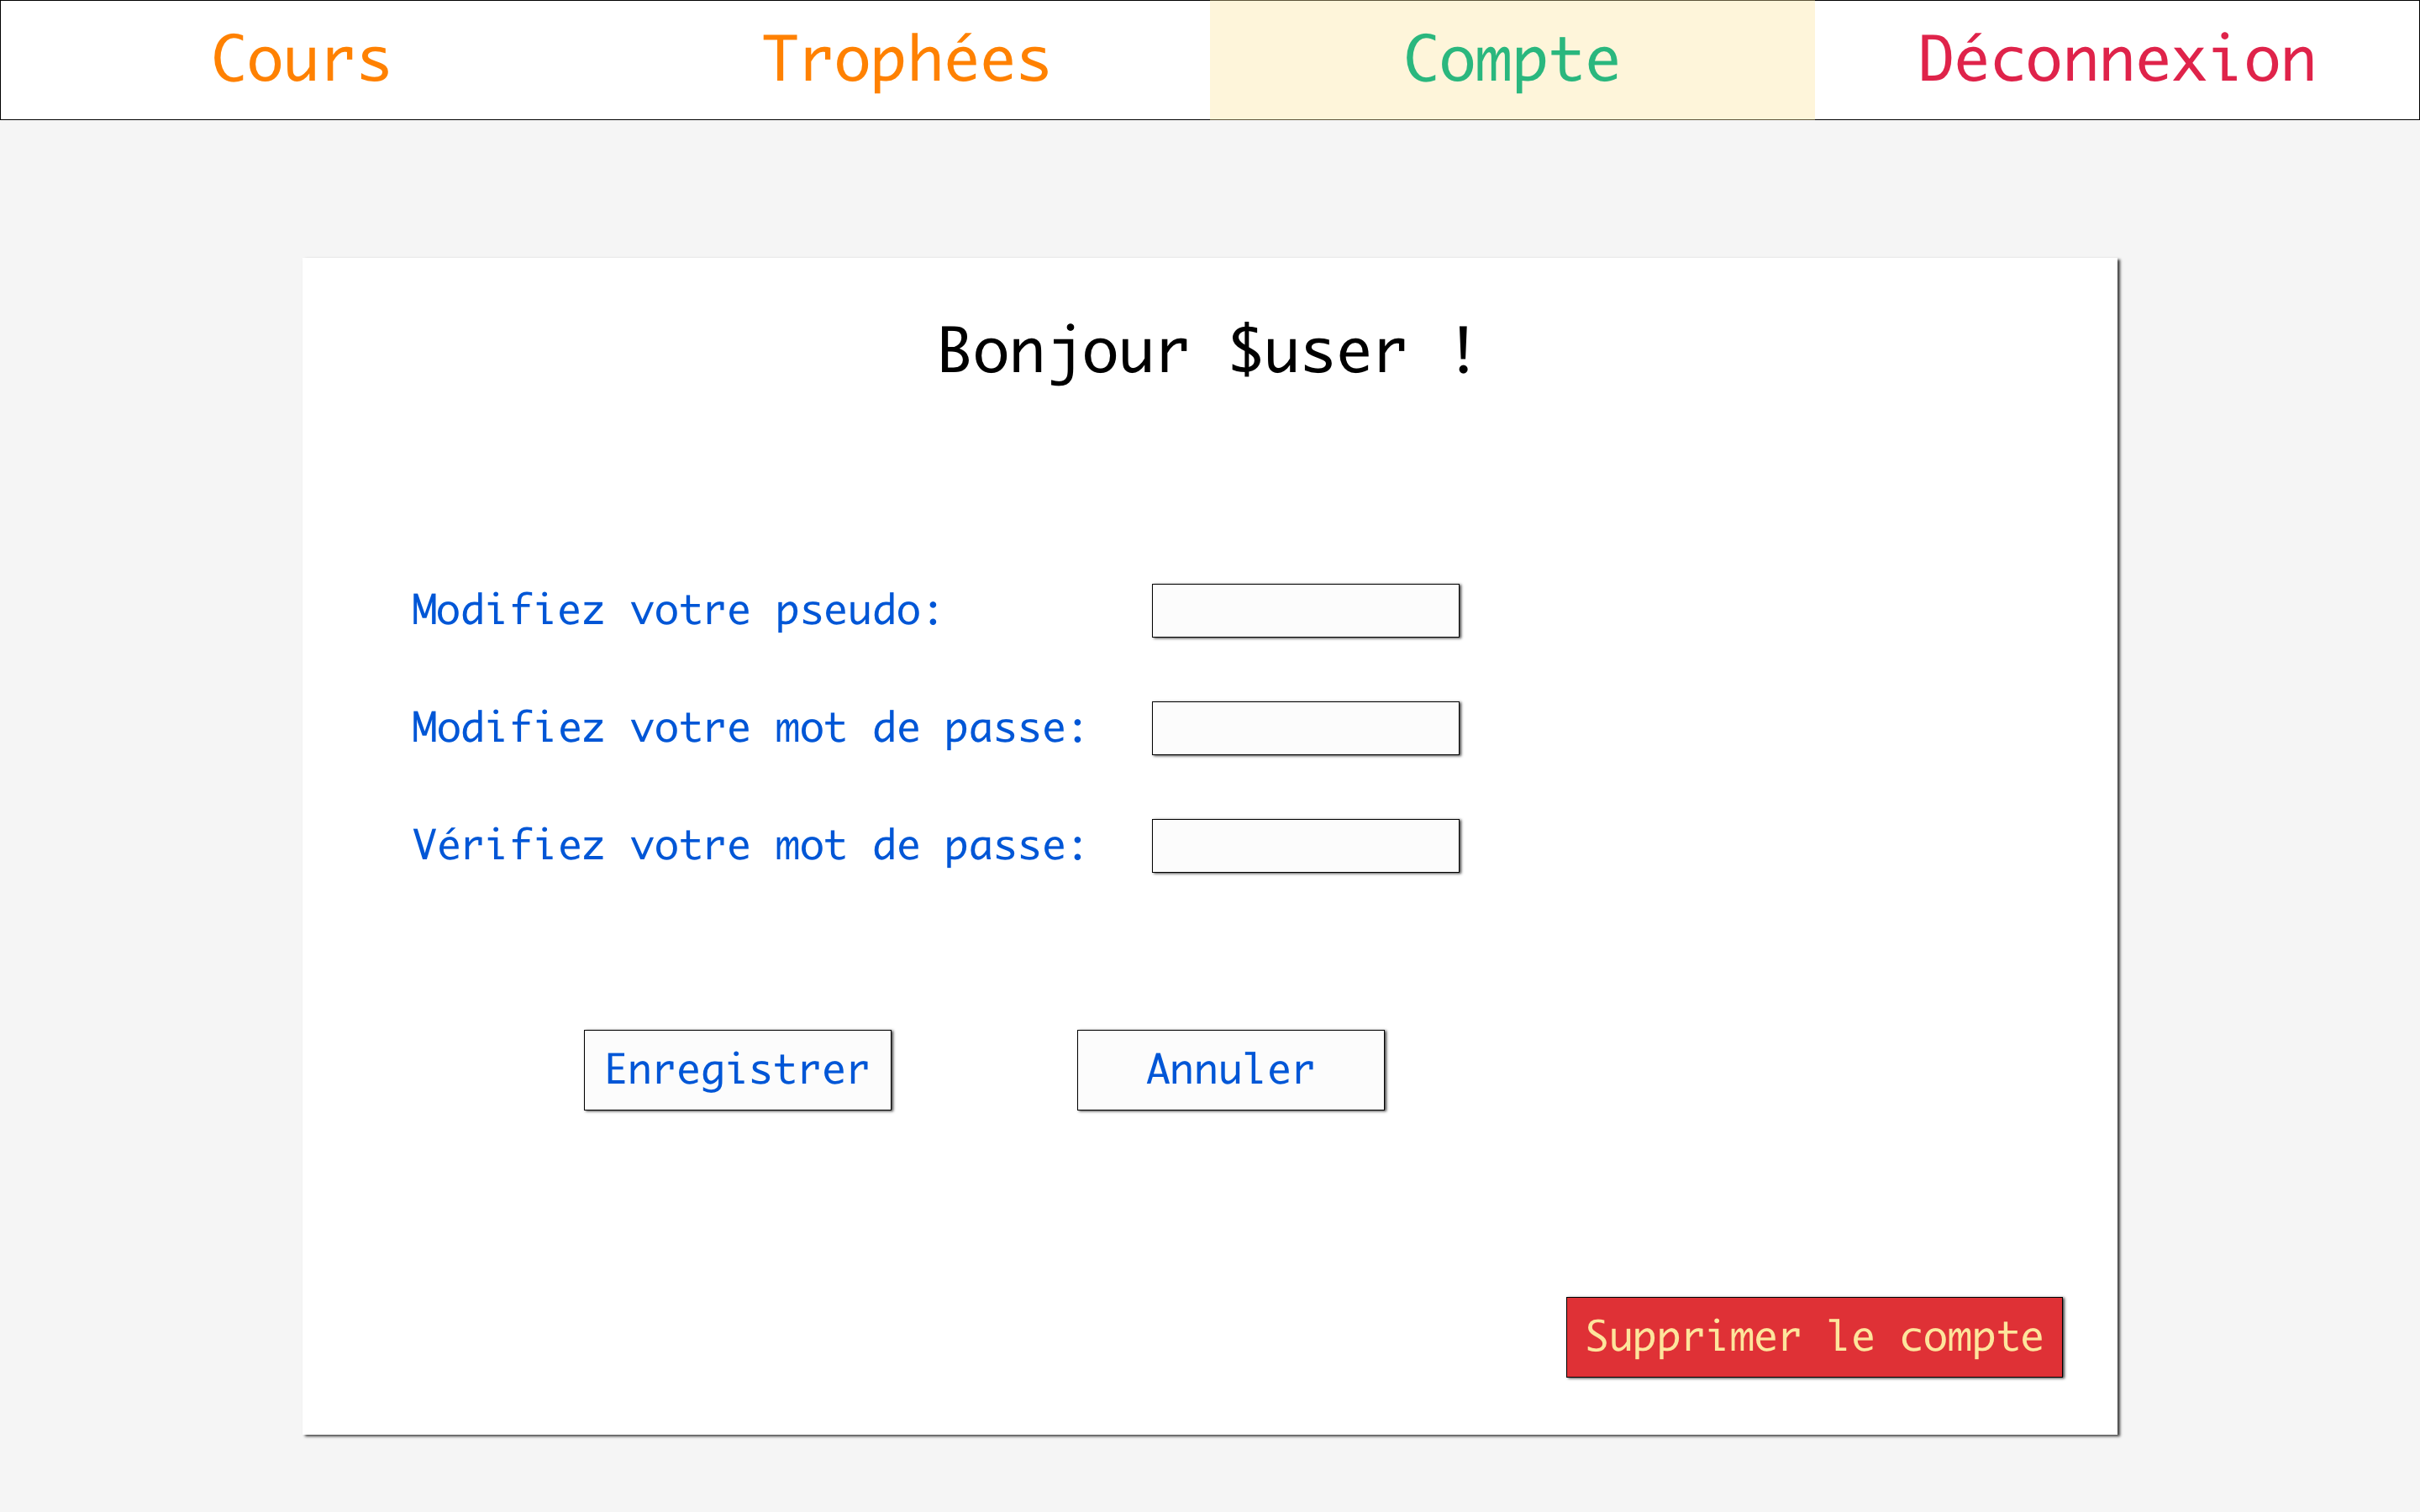
\includegraphics[scale=0.14]{textures/images/annexes/maquettes/4-Compte.png}
    \caption{La page du compte}
\end{figure}
\newpage
\section*{Le site}
\addcontentsline{ptc}{section}{Le site}
\label{sec:site}

Voici les différentes pages du site finalisé :

\begin{figure}[!h]
    \centering
    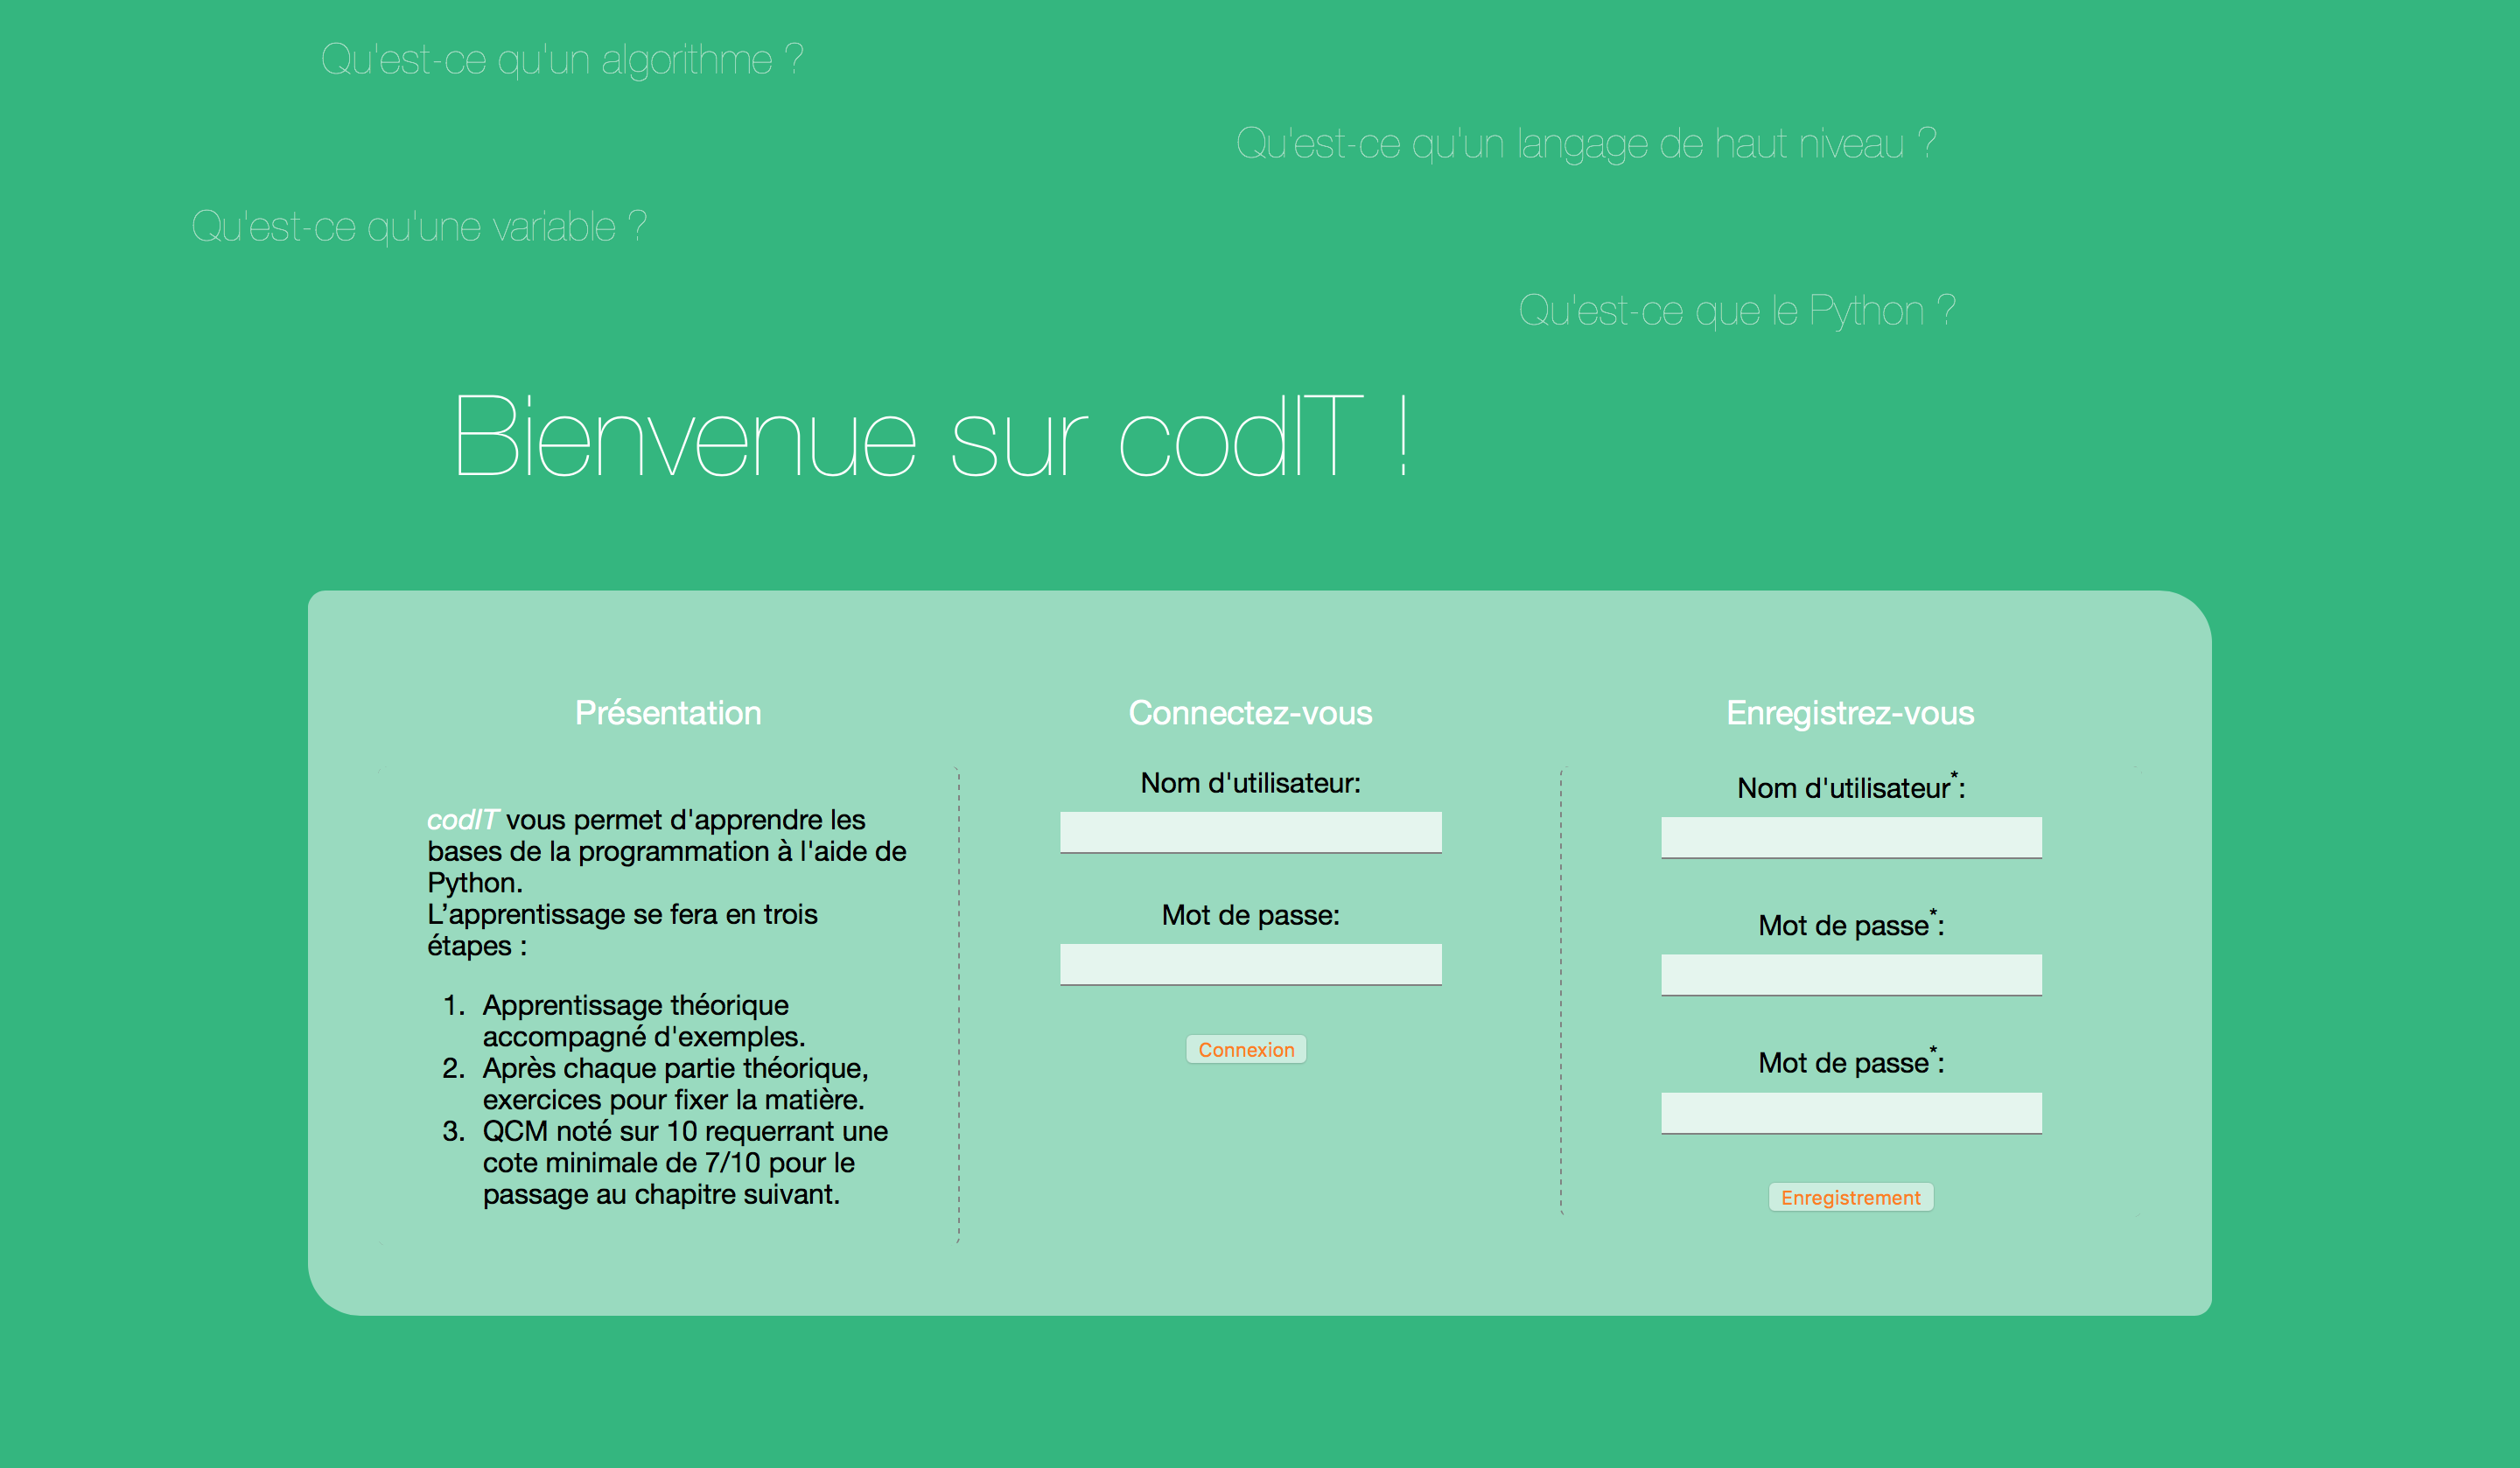
\includegraphics[scale=0.14]{textures/images/annexes/site/1-Login.png}
    \caption{La page d'accueil}
\end{figure}
\begin{figure}[!h]
    \centering
    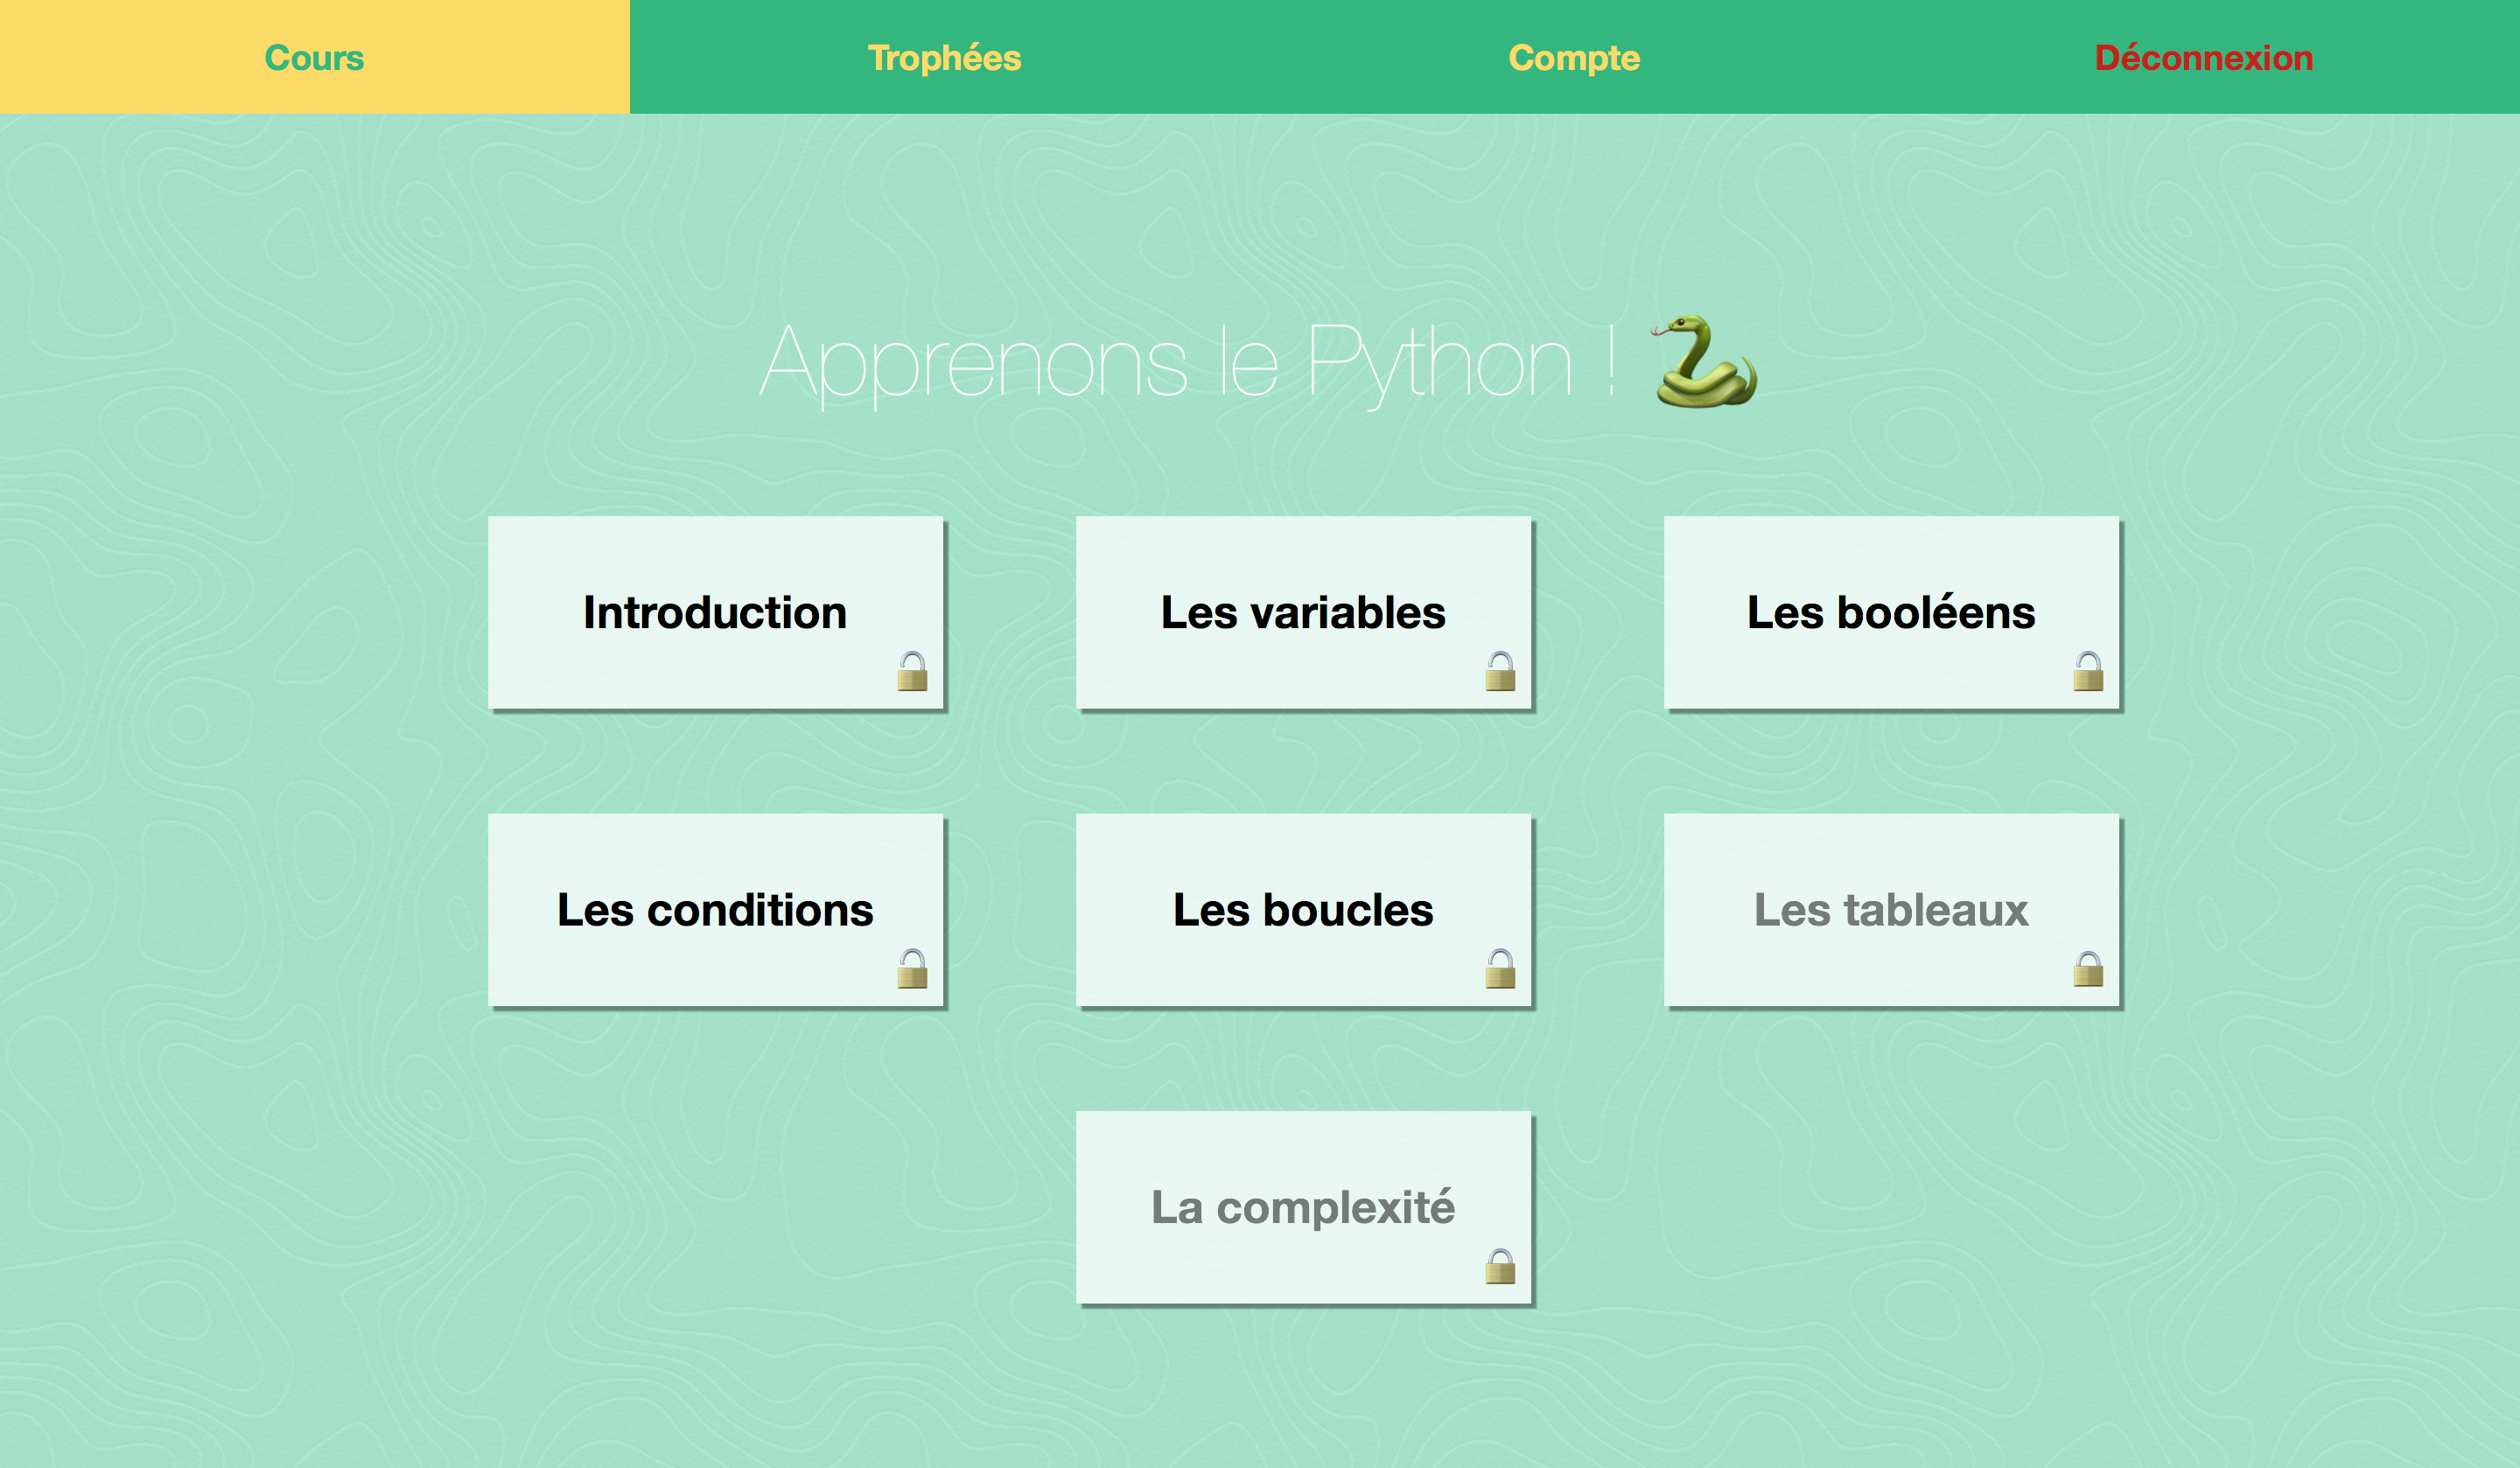
\includegraphics[scale=0.14]{textures/images/annexes/site/21-Sommaire.png}
    \caption{La page de cours}
\end{figure}

\newpage

\begin{figure}[!h]
    \centering
    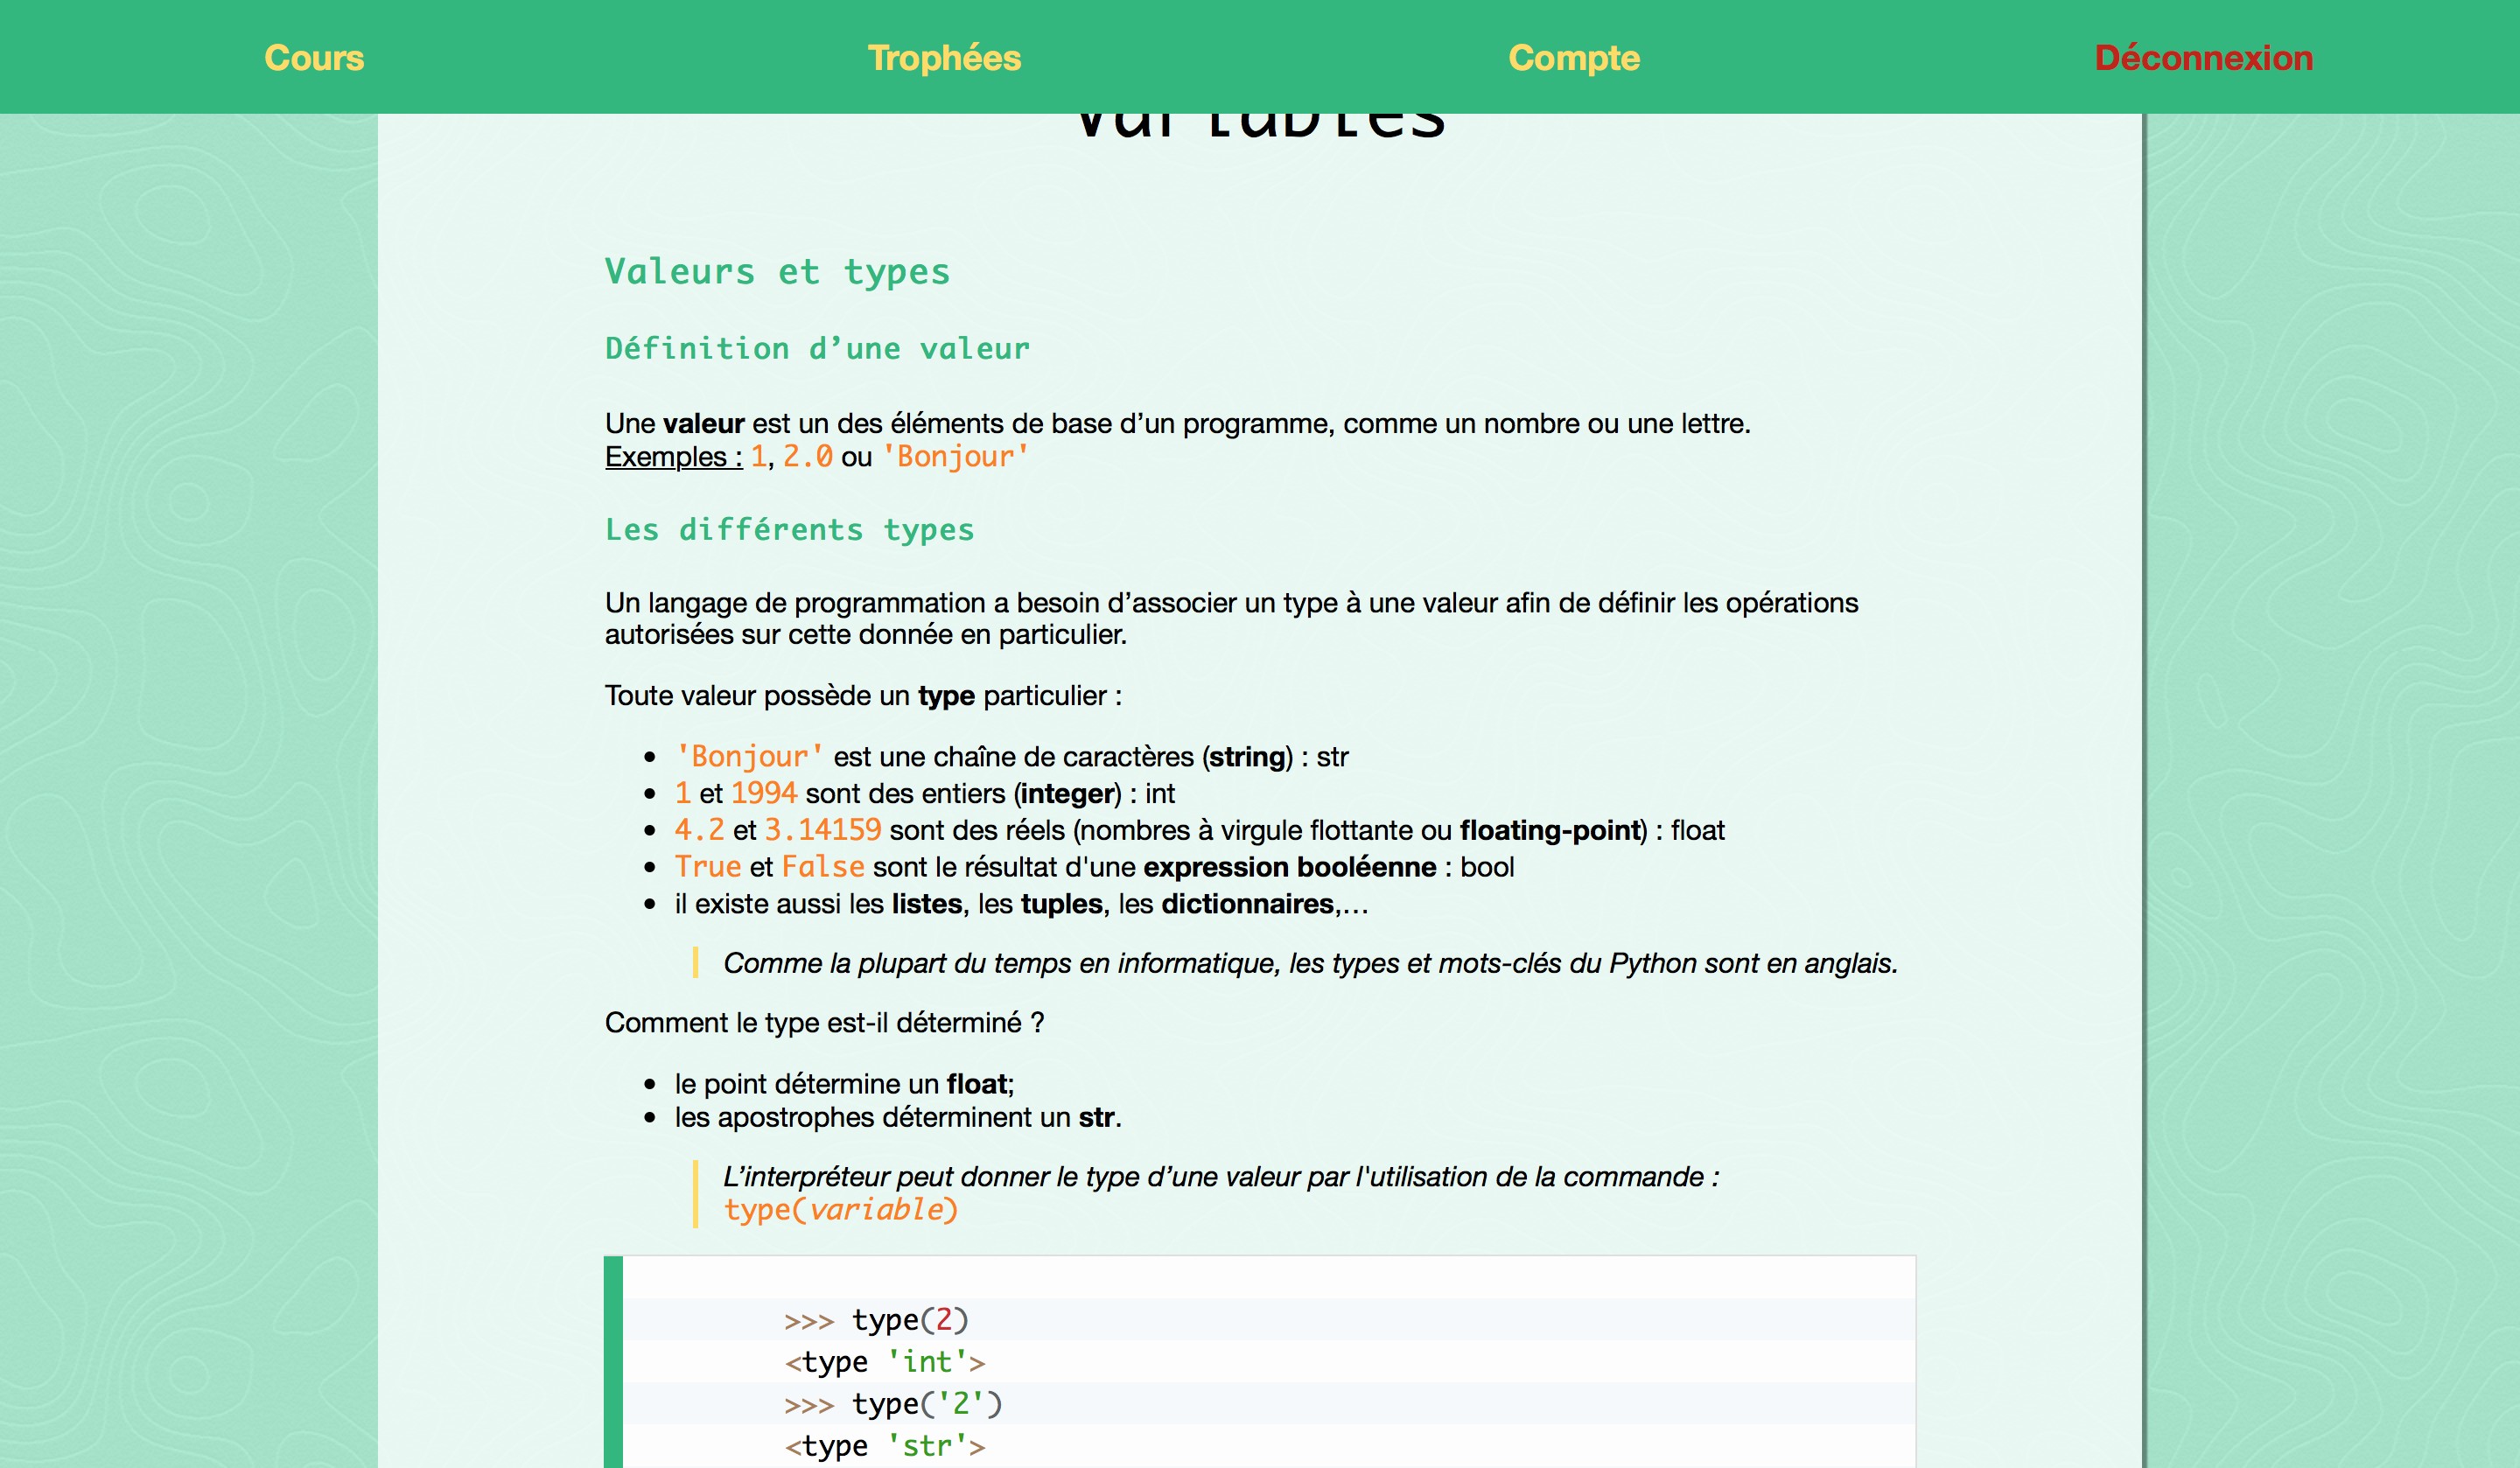
\includegraphics[scale=0.14]{textures/images/annexes/site/22-Cours.png}
    \caption{L'aperçu d'un chapitre}
\end{figure}
\begin{figure}[!h]
    \centering
    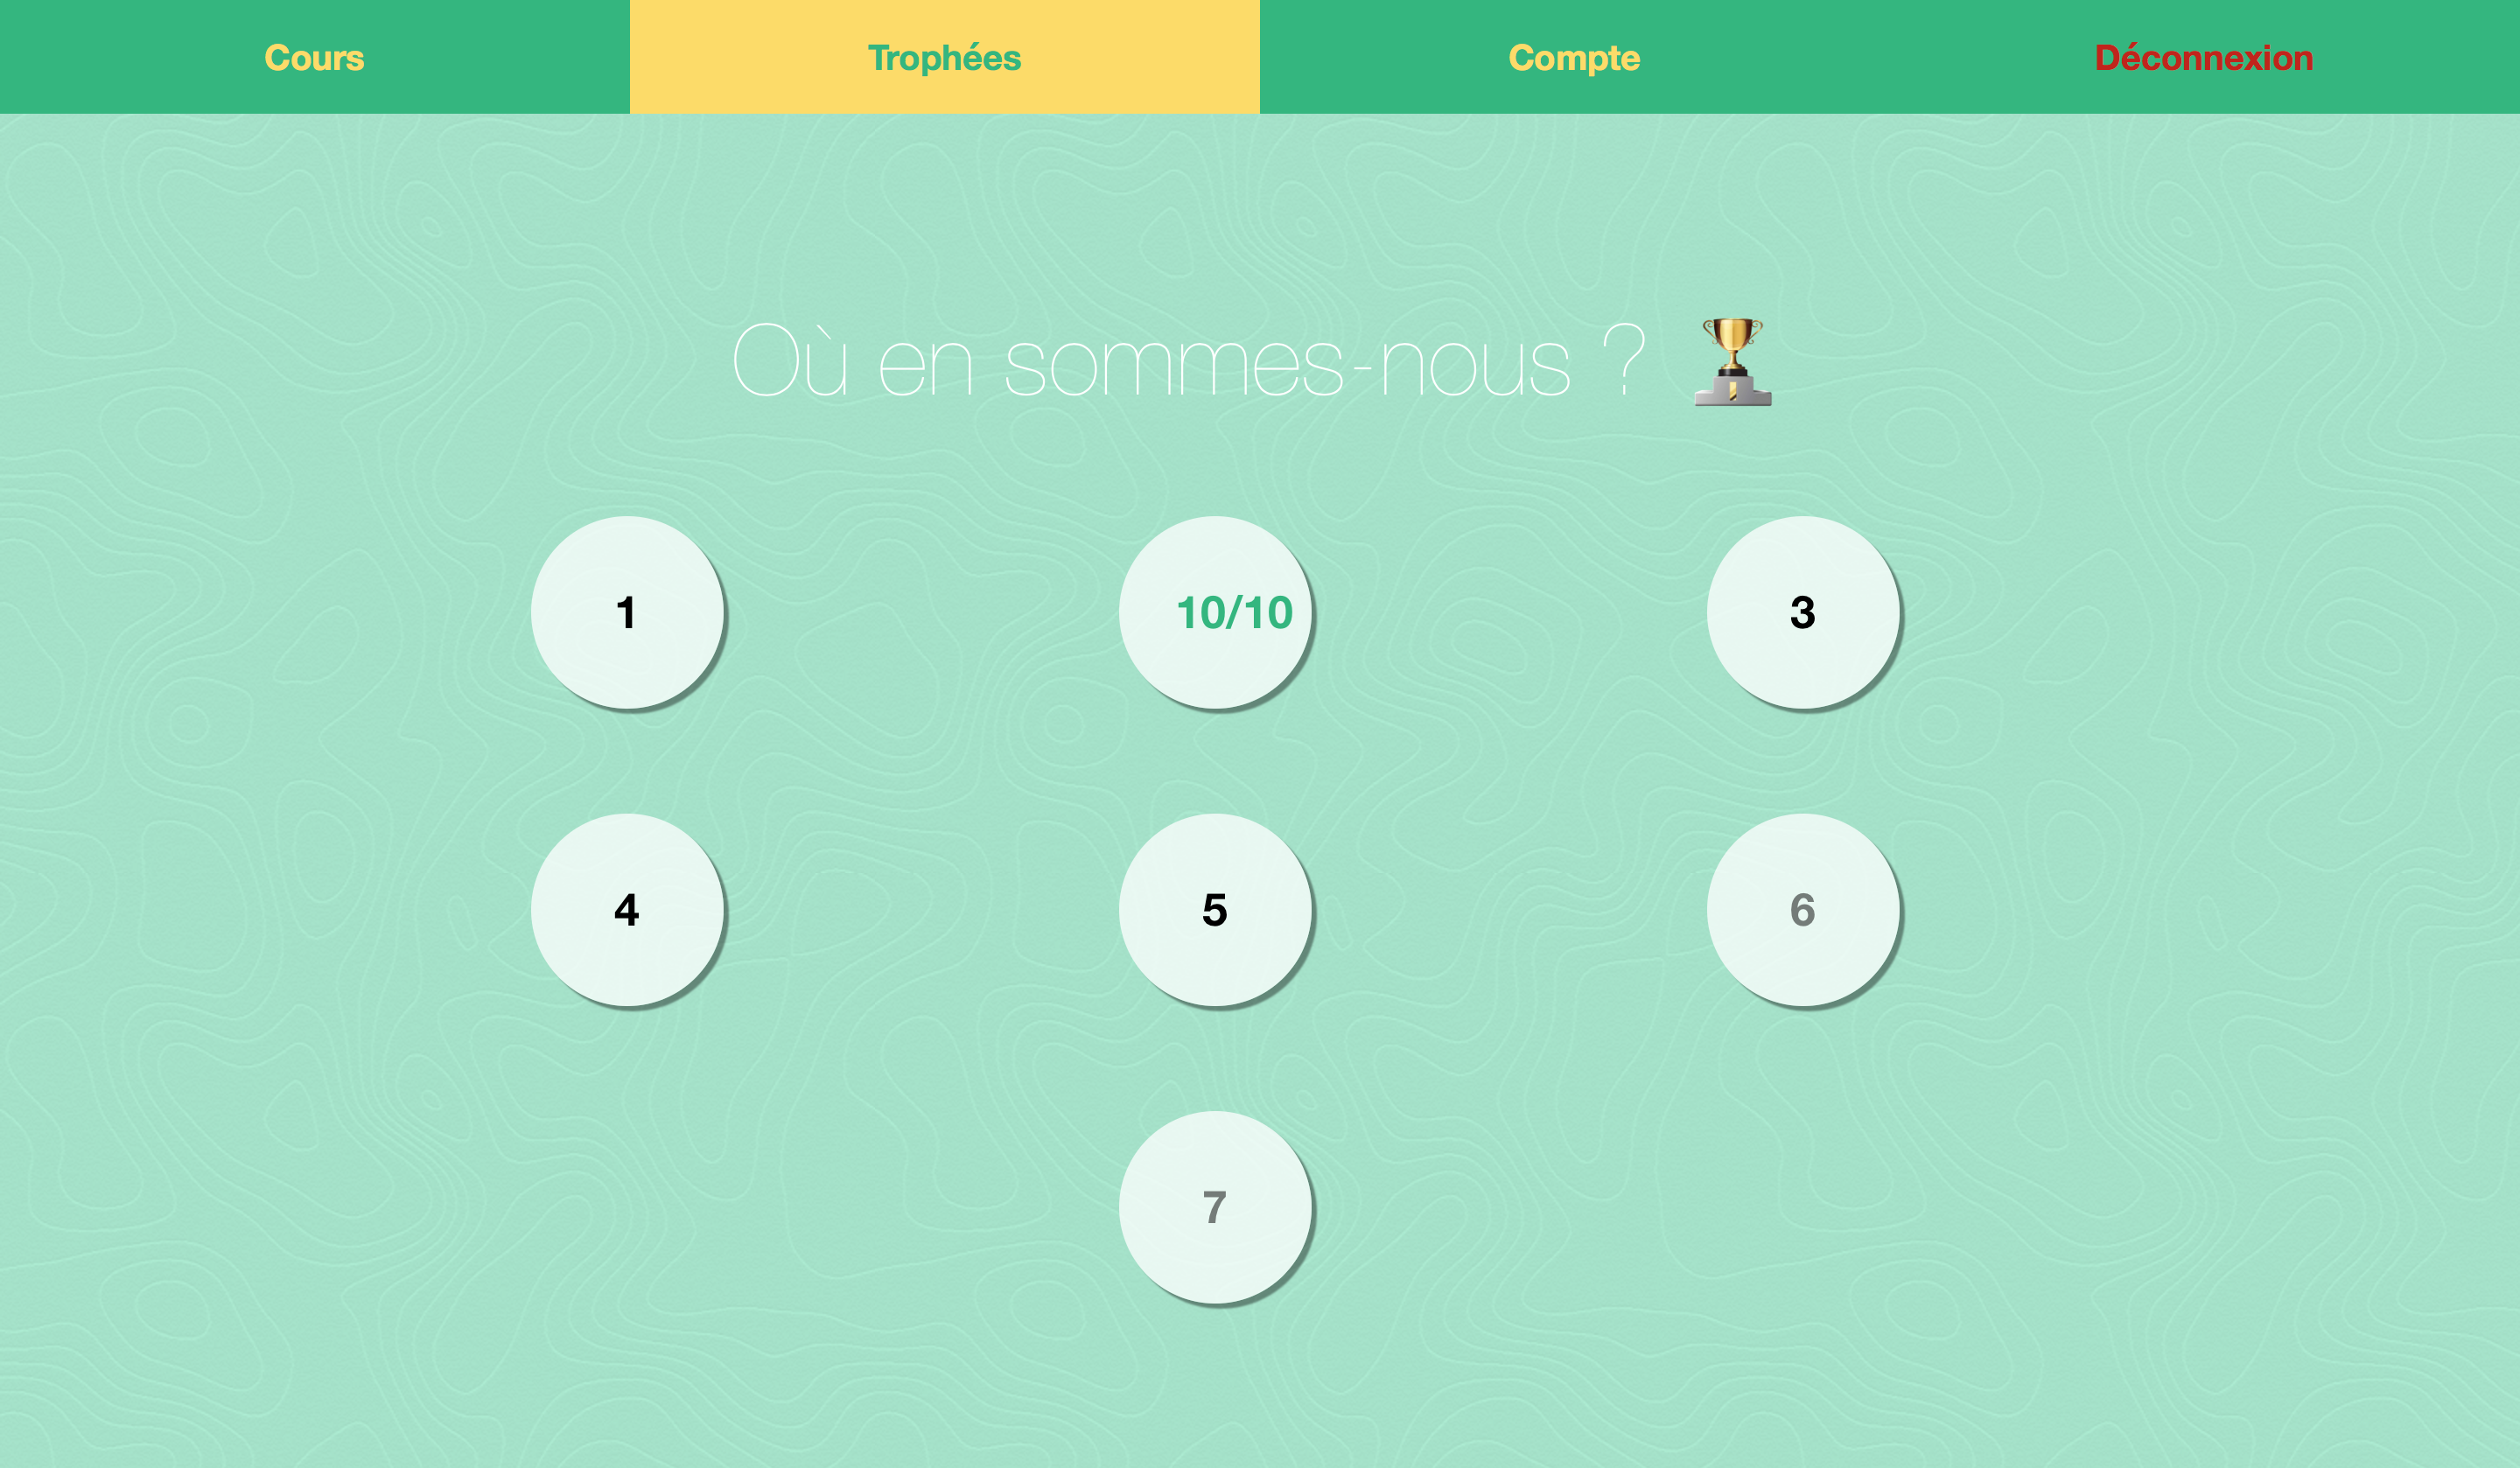
\includegraphics[scale=0.14]{textures/images/annexes/site/3-Trophees.png}
    \caption{La page des trophées}
\end{figure}

\newpage

\begin{figure}[!h]
    \centering
    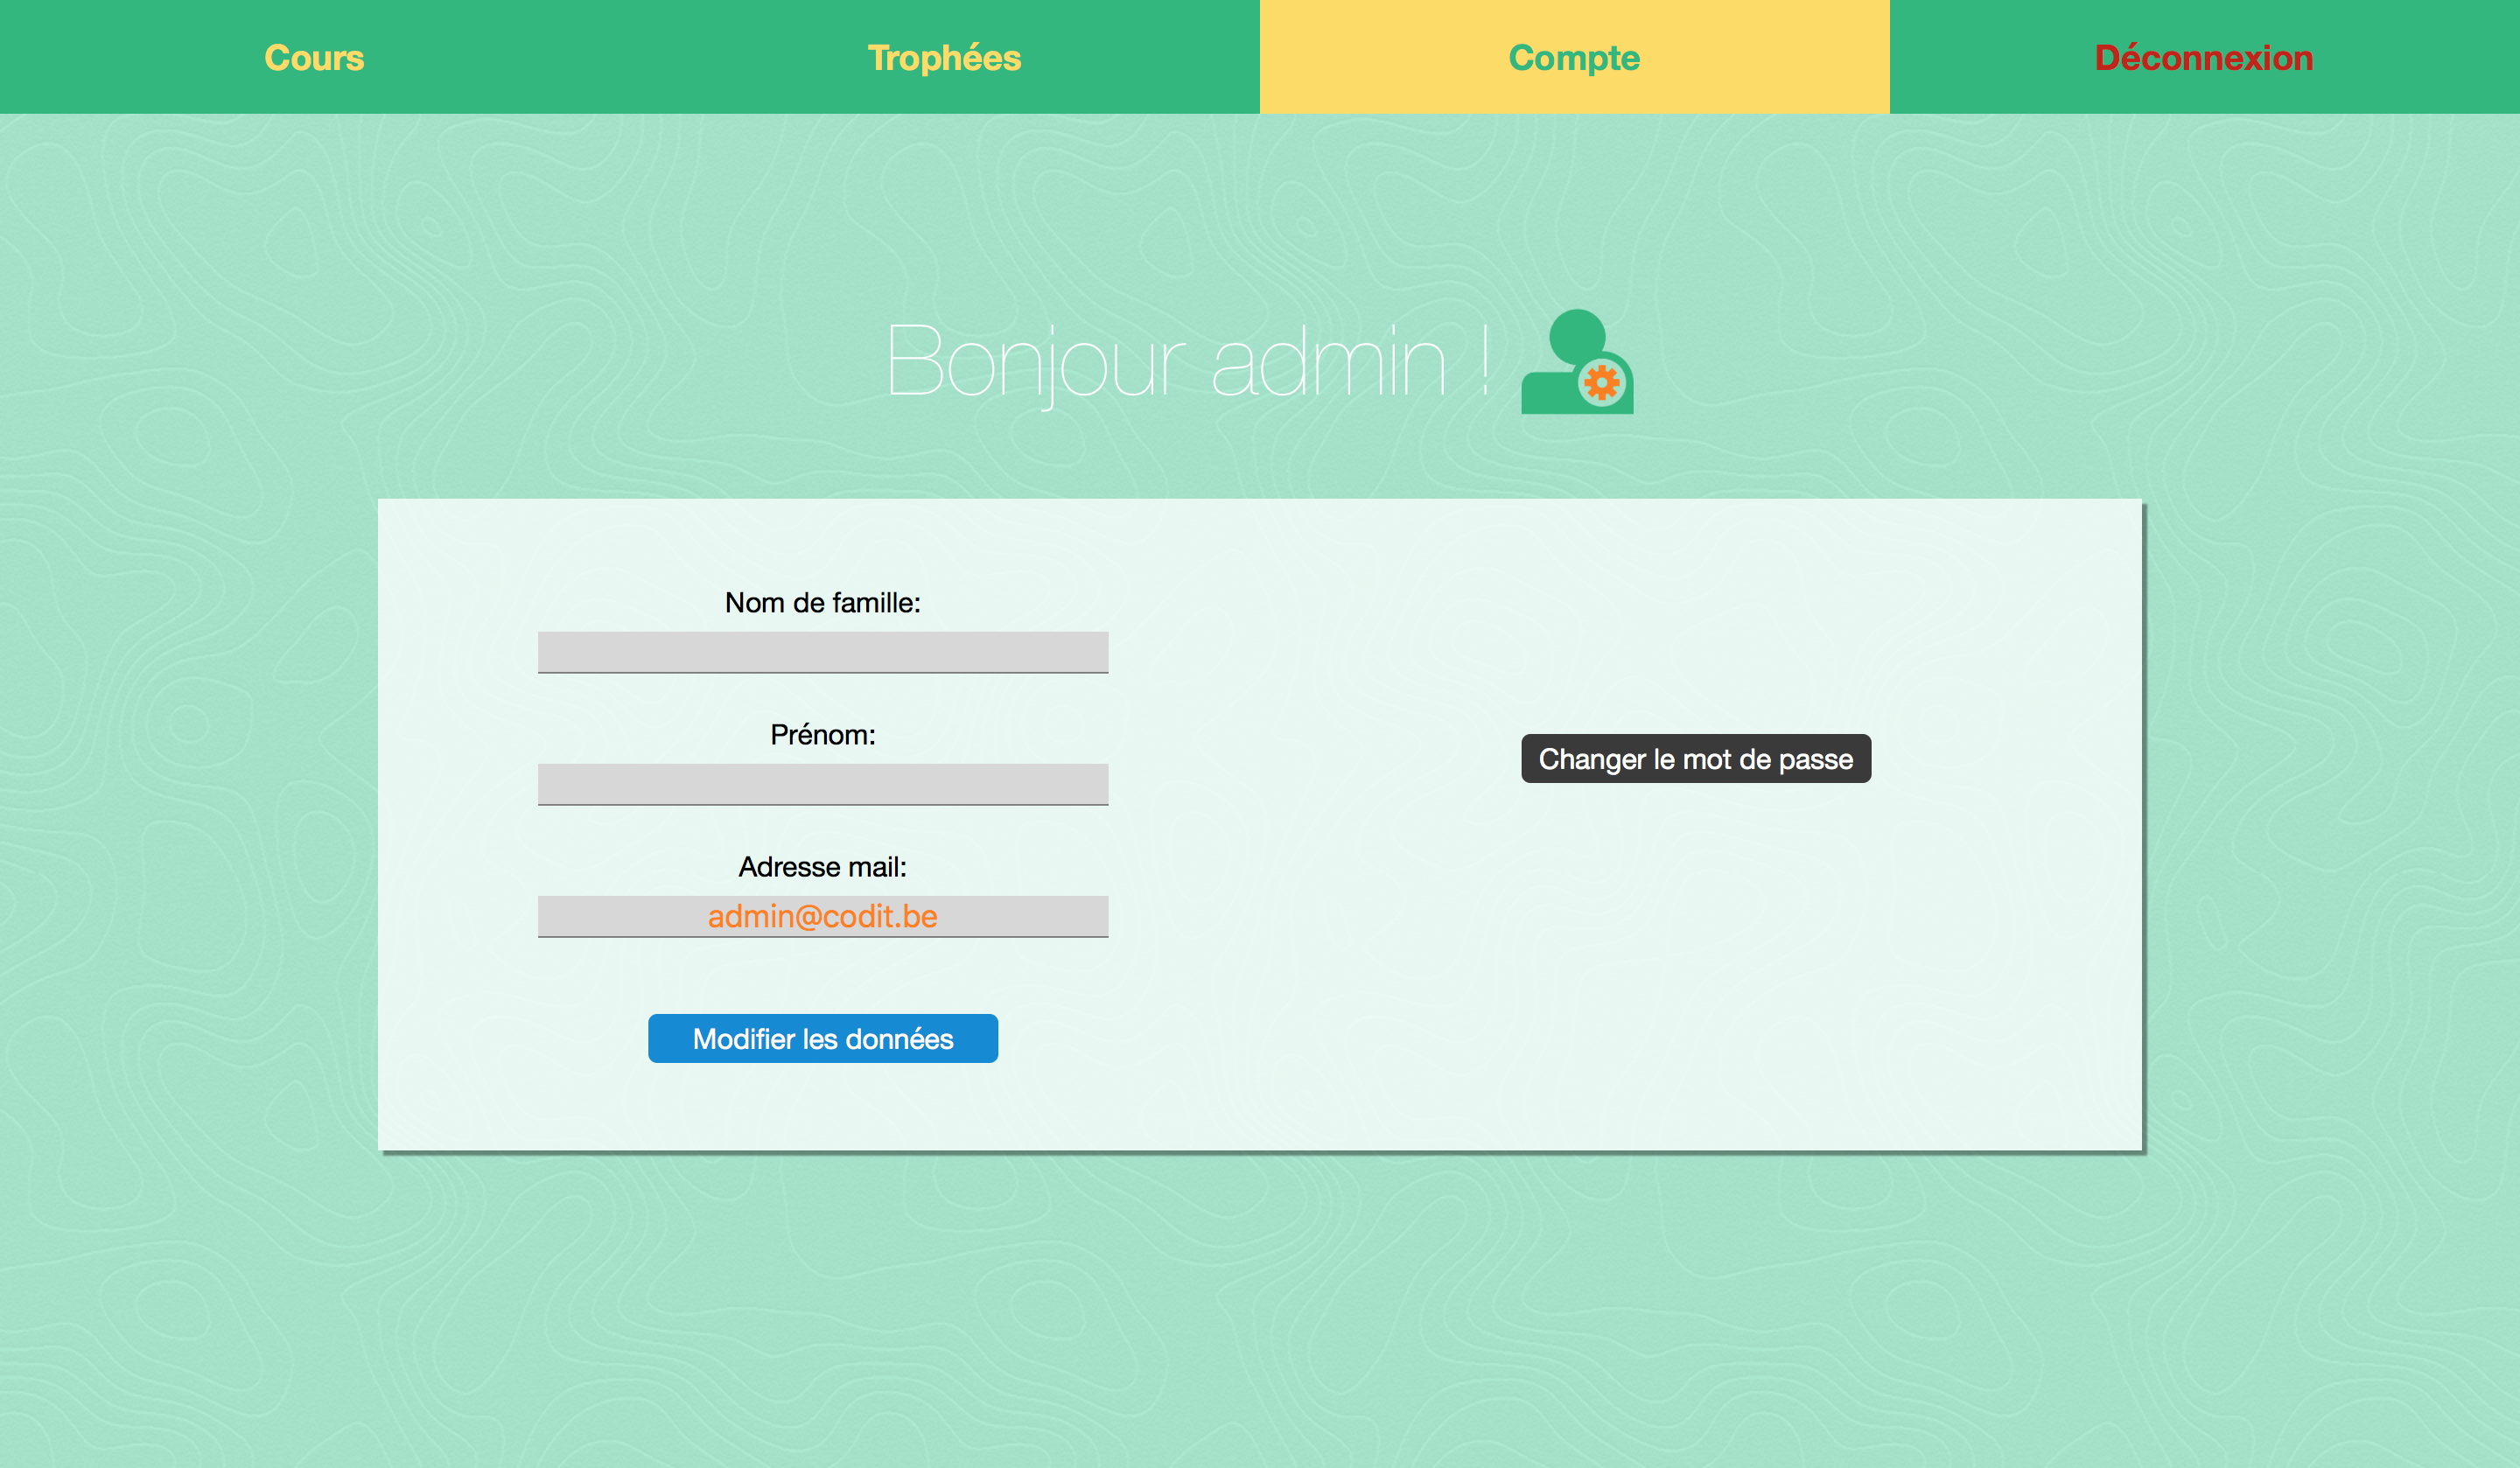
\includegraphics[scale=0.14]{textures/images/annexes/site/4-Compte.png}
    \caption{La page du compte}
\end{figure}

%%% Local Variables:
%%% mode: latex
%%% TeX-master: t
%%% End:
    \newpage
    \newpage
\thispagestyle{empty}
\setcounter{page}{0}
\null
\newpage
\end{document}
